
\scsection{Предметная область и онтология средств разработки ostis-систем}

\scsubsection{\textbf{Предметная область и онтология базовых интерпретаторов логико-семантических моделей ostis-систем}}
\label{sd_interpreters}
\begin{SCn}

\scnsectionheader{\currentname}
\scnstartsubstruct

\scnidtf{Предметная область и онтология платформ интерпретации sc-моделей компьютерных систем}
\scniselement{раздел базы знаний}
\scnrelfromlist{дочерний раздел}{\nameref{sd_program_interp};\nameref{sd_sem_comp}}

\scnheader{Предметная область базовых интерпретаторов логико-семантических моделей ostis-систем}
\scniselement{предметная область}
\scnsdmainclasssingle{платформа интерпретации sc-моделей компьютерный систем}
%\scnsdclass{***}
%\scnsdrelation{***}

\scnheader{логико-семантическая модель кибернетической системы}
\scnidtf{формальная модель (формальное описание) функционирования кибернетической системы, состоящая из:
	\begin{scnitemize}
		\item формальной модели информации, хранимой в памяти кибернетической системы;
		\item формальной модели коллектива агентов, осуществляющих обработку указанной информации.
\end{scnitemize}}
\scnsuperset{sc-модель кибернетической системы}
\scnaddlevel{1}
\scnidtf{логико-семантическая модель кибернетической системы, представленная в SC-коде}
\scnidtf{логико-семантическая модель ostis-системы, которая, в частности, может быть функционально эквивалентной моделью какой-либо кибернетической системы, не являющейся ostis-системой}
\scnaddlevel{-1}

\scnheader{кибернетическая система}
\scnsuperset{компьютерная система}
\scnaddlevel{1}
\scnidtf{искусственная кибернетическая система}
\scnsuperset ostis-система}
\scnaddlevel{1}
\scnidtf{компьютерная система, построенная по технологии OSTIS на основе интерпретации спроектированной логико-семантическая sc-модель этой системы}
\scnaddlevel{-2}

\scnheader{платформа интерпретации sc-моделей компьютерных систем}
\scnidtf{базовый интерпретатор логико-семантических моделей ostis-систем}
\scnidtf{Семейство платформ интерпретации sc-моделей компьютерных систем}
\scnidtf{платформа реализации sc-моделей компьютерных систем}
\scnidtftext{часто используемый sc-идентификатор}{универсальный интерпретатор sc-моделей компьютерных систем}
\scnidtf{универсальный интерпретатор унифицированных логико-семантических моделей компьютерных систем}
\scnsubset{встроенная ostis-система}
\scnidtf{встроенная пустая ostis-система}
\scnidtf{универсальный интерпретатор sc-моделей ostis-систем}
\scnidtf{универсальная базовая ostis-система, обеспечивающая имитацию любой ostis-системы путем интерпретации sc-модели имитируемой ostis-системы}
\scnnote{соотношение между имитируемой и универсальной ostis-системой в известной мере аналогично соотношению между машиной Тьюринга и универсальной машиной Тьюринга}
\scnexplanation{Под \textbf{\textit{платформой интерпретации sc-моделей компьютерных систем}} понимается реализация платформы интерпретации sc-моделей, которая в общем случае включает в себя:

Реализация \textit{платформы интерпретации sc-моделей компьютерных систем} (\textit{универсального интерпретатора sc-моделей компьютерных систем}) может иметь большое число вариантов -- как программно, так и аппаратно реализованных. Логическая архитектура \textit{платформы интерпретации sc-моделей компьютерных систем} обеспечивает независимость проектируемых компьютерных систем от многообразия вариантов реализации интерпретатора их моделей и в общем случае включает в себя:

\begin{scnitemize}
    \item хранилище \textit{sc-текстов} (\textit{sc-хранилище}, хранилище знаковых конструкций, представленных SC-коде);
    \item файловую память \textit{sc-машины};
    \item средства, обеспечивающие взаимодействие \textit{sc-агентов} над общей памятью (sc-памятью);
    \item базовые средства интерфейса для взаимодействия системы с внешним миром (пользователем или другими системами). Указанные средства включают в себя, как минимум, редактор, транслятор (в sc-память и из нее) и визуализатор для одного из базовых универсальных вариантов представления \textit{SC-кода} (\textit{SCg-код}, \textit{SCs-код}, \textit{SCn-код}), средства, позволяющие задавать системе вопросы из некоторого универсального класса (например, запрос семантической окрестности некоторого объекта);
    \item реализацию \textit{Абстрактной scp-машины}, то есть интерпретатор \textit{scp-программ} (программ Языка SCP).
\end{scnitemize}
При необходимости, в \textbf{\textit{платформу интерпретации sc-моделей компьютерных систем}} могут быть заранее на платформенно-зависимом уровне включены какие-либо компоненты машин обработки знаний или баз знаний, например, с целью упрощения создания первой версии \textit{прикладной ostis-системы}.

Реализация платформы может осуществляться на основе произвольного набора существующих технологий, включая аппаратную реализацию каких-либо ее частей. С точки зрения компонентного подхода любая \textbf{\textit{платформа интерпретации sc-моделей компьютерных систем}} является \textbf{\textit{платформенно-зависимым многократно используемым компонентом}}.}
\scnsuperset{программный вариант реализации платформы интерпретации sc-моделей компьютерных систем}
\scnsuperset{семантический ассоциативный компьютер}
\scnsubdividing{однопользовательский вариант реализации платформы интерпретации sc-моделей компьютерных систем\\
	\scnaddlevel{1}
		\scnidtf{вариант реализации платформы интерпретации sc-моделей компьютерных систем, рассчитанный на то, что с конкретной ostis-системой взаимодействует только один пользователь (владелец)}
		\scnnote{При таком варианте реализации платформы оказывается невозможным реализовать некоторые важные принципы \textit{Технологии OSTIS}, например, коллективную согласованную разработку базы знаний системы в процессе ее эксплуатации. При этом могут использоваться различные сторонние средства, например для разработки базы знаний на уровне исходных текстов.}
	\scnaddlevel{-1}
;многопользовательский вариант реализации платформы интерпретации sc-моделей компьютерных систем\\
\scnaddlevel{1}
	\scnidtf{вариант реализации платформы интерпретации sc-моделей компьютерных систем, рассчитанный на то, что с конкретной ostis-системой одновременно или в разное время могут взаимодействовать разные пользователи, в общем случае обладающие разными правами, сферами ответственности, уровнем опыта, и имеющие свою конфиденциальную часть хранимой в базе знаний информации}
\scnaddlevel{-1}}

\scnheader{платформа интерпретации sc-моделей компьютерных систем}
\scnsubdividing{программный вариант реализации платформы интерпретации sc-моделей компьютерных систем\\
	\scnaddlevel{1}
	\scnidtf{программная платформа интерпретации sc-моделей ostis-систем}
	\scnidtf{программный базовый интерпретатор sc-моделей ostis-систем}
	\scnaddlevel{-1}
	;семантический ассоциативный компьютер
	\scnaddlevel{1}
	\scnidtf{аппаратная платформа интерпретации sc-моделей ostis-систем}
	\scnidtf{аппаратно реализованный базовый интерпретатор sc-моделей ostis-систем}
	\scnaddlevel{-1}
}

\scnheader{cистема управления базами данных}
\scnidtf{комплекс программ, позволяющих создать базу данных (БД) и манипулировать данными (вставлять, обновлять, удалять и выбирать)}
\scnsubdividing{NoSQL СУБД\\
	\scnaddlevel{1}
	\scnidtf{графовая система управления базами данных}
	\scnidtf{это подход к реализации масштабируемого хранилища (базы) информации с гибкой моделью данных, отличающийся от классических реляционных СУБД}
	\scnhaselement{Neo4j}
	\scnhaselement{Redis}
	\scnhaselement{Apache Cassandra}
	\scnaddlevel{-1}
	;SQL СУБД\\
	\scnaddlevel{1}
	\scnidtf{реляционная система управления базами данных}
	\scnidtf{ это язык структурированных запросов, позволяющий хранить, манипулировать и извлекать данные из реляционных баз данных}
	\scnhaselement{PostgreSQL}
	\scnhaselement{MySQL}
	\scnhaselement{Oracle}
	\scnaddlevel{-1}
	\scnreltolist{ключевой знак} {\scncite{Neo4j};\scncite{Redis};\scncite{Apache Cassandra};\scncite{PostgreSQL};\scncite{MySQL};\scncite{Oracle}}
}

\scnmakeset{NoSQL СУБД;SQL СУБД}

\scntext{сравнение}{Графовые СУБД имеют ряд выгодных отличий от реляционных СУБД, важнейшими из которых являются:
	\begin{scnitemize}
		
		\item гибкость - типология связей между сущностями и вообще структура БД может свободно меняться в любой момент, каждый объект может обладать произвольным количеством связей с другими объектами;
		
		\item минимизация дублирований и локализация изменений - поскольку БД обладает гибкой нелинейной структурой, каждый объект в БД достаточно указать один раз. Как следствие, изменения в такой БД легко локализуются.
		
	\end{scnitemize}
	Тем не менее, несмотря на указанные достоинства, графовые СУБД все еще используются в реальных проектах значительно реже, чем традиционные реляционные СУБД. Это обусловлено следующими недостатками:
	
	\begin{scnitemize}
		
		\item поиск в графовой СУБД в общем случае выполняется более медленно и в гораздо большей степени зависит от объема базы данных, чем в реляционной БД. Это связано с тем, что:
		
		\begin{scnitemizeii}
			
			\item поиск в графе произвольной структуры в принципе является алгоритмически сложной задачей, реляционная БД в данном случае выигрывает за счет более четкой структуры;
			
			\item независимо от способа хранения данных все графовые СУБД в конечном счете реализуются на современных аппаратных средствах, которые имеют линейную структуру памяти и изначально не предназначены для хранения и обработки нелинейных (графовых) конструкций. Это приводит к значительным накладным расходам по преобразованию графа к линейному способу хранения, необходимости оптимизации соответствующих алгоритмов и т.д.
			
		\end{scnitemizeii}
		
		\item строгая структура реляционных БД позволяет более четко описать критерии и отслеживать целостность БД. В графовых СУБД целостность информации по умолчанию не гарантируется, а достигается дополнительными средствами анализа БД. В общем случае для обеспечения целостности и вообще качества графовой БД необходимо учитывать семантику (смысл) представляемой информации, однако в подавляющем большинстве современных графовых СУБД данный вопрос практически не рассматривается.
	\end{scnitemize}
}

\bigskip

\scnendstruct \scnendcurrentsectioncomment

\end{SCn}

\scsubsubsection{Предметная область и онтология программных вариантов реализации базового интерпретатора логико-семантических моделей ostis-систем на современных компьютерах}
\label{sd_program_interp}
\begin{SCn}
	
\scnsectionheader{\currentname}
\scnstartsubstruct

\scnheader{Предметная область программных вариантов реализации базового интерпретатора логико-семантических моделей ostis-систем на современных компьютерах}
\scniselement{предметная область}
\scnsdmainclasssingle{программный вариант реализации платформы интерпретации sc-моделей компьютерных систем}
\scnhaselementlist{ключевой объект исследования}{Программный вариант реализации платформы интерпретации sc-моделей компьютерных систем;Программная модель sc-памяти;Реализация sc-хранилища и средств доступа к нему;Реализация sc-хранилища;sc-адрес;элемент sc-хранилища;метка синтаксического типа sc-элемента;метка уровня доступа sc-элемента;sc-итератор;sc-шаблон;контекст процесса в рамках программной модели sc-памяти;блокировка sc-элемента в рамках программной модели sc-памяти;подписка на событие в sc-памяти в рамках программной модели sc-памяти;Реализация файловой памяти ostis-системы;Реализация базового набора платформенно-зависимых sc-агентов и их компонентов;Реализация подсистемы взаимодействия с внешней средой с использованием сетевых протоколов;SCTP;sctp-команда;Реализация подсистемы взаимодействия с внешней средой с использованием протоколов SCTP;Реализация подсистемы взаимодействия с внешней средой с использованием протоколов на основе формата JSON;Реализация вспомогательных инструментальных средств для работы c sc-памятью;Реализация интерпретатора sc-моделей пользовательских интерфейсов;Реализация scp-интерпретатора}

\scnheader{программный вариант реализации платформы интерпретации sc-моделей компьютерных систем}
\scnidtf{программная реализация платформы интерпретации sc-моделей компьютерных систем }
\scnidtf{программный вариант реализации базового интерпретатора логико-семантических моделей компьютерных систем}
\scnidtf{программный вариант реализации базового интерпретатора логико-семантических моделей ostis-систем на современных компьютерах}
\scnidtf{вариант реализации базового интерпретатора логико-семантических моделей компьютерных систем на традиционных компьютерах с архитектурой фон Неймана}
\scnexplanation{Одним из путей, позволяющих осуществлять апробацию, развитие, а в ряде случаев и внедрение новых моделей и технологий вне зависимости от наличия соответствующих аппаратных средств является разработка программных моделей этих аппаратных средств, которые были бы функционально эквивалентны этим аппаратным средствам, но при этом интерпретировались на базе традиционной аппаратной архитектуры (в данной работе традиционной архитектурой будем считать архитектуру фон Неймана, как доминирующую в настоящее время). Очевидно, что производительность таких программных моделей в общем случае будет ниже, чем самих аппаратных решений, однако в большинстве случаев она оказывается достаточной для того, чтобы развивать соответствующую технологию параллельно с разработкой аппаратных средств и осуществления постепенного перевода уже работающих систем с программной модели на аппаратные средства.}
\scnsuperset{web-ориентированный вариант реализации платформы интерпретации sc-моделей компьютерных систем}
\scnaddlevel{1}
	\scnidtf{вариант реализации платформы интерпретации sc-моделей компьютерных систем предполагающий взаимодействие пользователей с системой посредством сети Интернет}
	\scnsubset{многопользовательский вариант реализации платформы интерпретации sc-моделей компьютерных систем}
	\scnhaselement{Программный вариант реализации платформы интерпретации sc-моделей компьютерных систем}
\scnaddlevel{-1}

\scnheader{Программный вариант реализации платформы интерпретации sc-моделей компьютерных систем}
\scntext{принципы реализации}{Поскольку sc-тексты представляют собой семантические сети, то есть, по сути, графовые конструкции определенного вида, то на нижнем уровне задача разработки программного варианта реализации платформы интерпретации sc-моделей сводится к разработке средств хранения и обработки таких графовых конструкций.
	
	К настоящему времени разработано большое количество простейших моделей представления графовых конструкций в линейной памяти, таких как матрицы смежности, списки смежности и другие \scncite{Diskrete_Math}. Однако, при разработке сложных систем как правило приходится использовать более эффективные модели, как с точки зрения объема информации, требуемого для представления, так и с точки зрения эффективности обработки графовых конструкций, хранимых в той или иной форме.
	
	К наиболее распространенным программным средствам, ориентированным на хранение и обработку графовых конструкций относятся графовые СУБД (Neo4j \scncite{Neo4j}, ArangoDB \scncite{ArangoDB}, OrientDB \scncite{OrientDB}, Grakn \scncite{Grakn} и др.), а также так называемые rdf-хранилища (Virtuoso \scncite{Virtuoso}, Sesame \scncite{Sesame} и др.), предназначенные для хранения конструкций, представленных в модели RDF. Для доступа к информации, хранимой в рамках таких средств, могут использоваться как языки, реализуемые в рамках конкретного средства (например, язык Cypher в Neo4j), так и языки, являющиеся стандартами для большого числа систем такого класса (например, SPARQL для rdf-хранилищ).
	
	Популярность и развитость такого рода средств приводит к тому, что на первый взгляд целесообразным и эффективным кажется вариант реализации \textit{программного варианта реализации платформы интерпретации sc-моделей} на базе одного из таких средств. Однако, существует ряд причин, по которым было принято решение о реализации \textit{программного варианта реализации платформы интерпретации sc-моделей} с нуля. К ним относятся следующие:
	
	\begin{scnitemize}
		\item для обеспечения эффективности хранения и обработки информационных конструкций определенного вида (в данном случае -- конструкций SC-кода, sc-конструкций), должна учитываться специфика этих конструкций. В частности, описанные в работе \scncite{Koronchik2013} эксперименты показали значительный прирост эффективности собственного решения по сравнению с существующими на тот момент;
		\item в отличие от классических графовых конструкций, где дуга или ребро могут быть инцидентны только вершине графа (это справедливо и для rdf-графов) в SC-коде вполне типичной является ситуация, когда sc-коннектор инцидентен другому sc-коннектору или даже двум sc-коннекторам. В связи с этим существующие средства хранения графовых конструкций не позволяют в явном виде хранить sc-конструкции (sc-графы). Возможным решением данной проблемы является переход от sc-графа к орграфу инцидентности, пример которого описан в работе \scncite{Ivashenko2015}, однако такой вариант приводит к увеличению числа хранимых элементов в несколько раз и значительно снижает эффективность алгоритмов поиска из-за необходимости делать большое количество дополнительных итераций;
		\item в основе обработки информации в рамках Технологии OSTIS лежит многоагентный подход, в рамках которого агенты обработки информации, хранимой в sc-памяти (sc-агенты) реагируют на события, происходящие в sc-памяти и обмениваются информацией посредством спецификации выполняемых ими действий в sc-памяти \scncite{Shunkevich2018}. В связи с этим одной из важнейших задач является реализация в рамках \textit{программного варианта реализации платформы интерпретации sc-моделей} возможности подписки на события, происходящие в программной модели sc-памяти, которая на данный момент практически не поддерживается в рамках современных средств хранения и обработки графовых конструкций;
		\item SC-код позволяет описывать также внешние информационные конструкции любого рода (изображения, текстовые файла, аудио- и видеофайлы и т.д.), которые формально трактуются как содержимое \textit{sc-элементов}, являющихся знаками \textit{внешних файлов ostis-системы}. Таким образом, компонентом \textit{программного варианта реализации платформы интерпретации sc-моделей} должна быть реализация файловой памяти, которая позволяет хранить указанные конструкции в каких-либо общепринятых форматах. Реализация такого компонента в рамках современных средств хранения и обработки графовых конструкций также не всегда представляется возможной.
	\end{scnitemize}
	
	По совокупности перечисленных причин было принято решение о реализации \textit{программного варианта реализации платформы интерпретации sc-моделей} "с нуля"{} с учетом особенностей хранения и обработки информации в рамках Технологии OSTIS.}
\scnrelfromset{декомпозиция программной системы}{Программная модель sc-памяти;Реализация интерпретатора sc-моделей пользовательских интерфейсов}
\scnexplanation{Текущий \textit{Программный вариант реализации платформы интерпретации sc-моделей компьютерных систем} является web-ориентированным, то есть с точки зрения современной архитектуры каждая ostis-система представляет собой web-сайт доступный онлайн посредством обычного браузера. Такой вариант реализации обладает очевидным преимуществом -- доступ к системе возможен из любой точки мира, где есть Интернет, при этом для работы с системой не требуется никакого специализированного программного обеспечения. С другой стороны, такой вариант реализации обеспечивает возможность параллельной работы с системой нескольких пользователей.

В то же время, взаимодействие клиентской и серверной части организовано таким образом, что web-интерфейс может быть легко заменен на настольный или мобильный интерфейс, как универсальный, так и специализированный.

Данный вариант реализации распространяется под open-source лицензией, для хранения исходных текстов используется хостинг Github и коллективная учетная запись ostis-dev.

Реализация является кроссплатформенной и может быть собрана из исходных текстов в различных операционных системах.}
\scnrelfrom{иллюстрация}{\scnfileimage{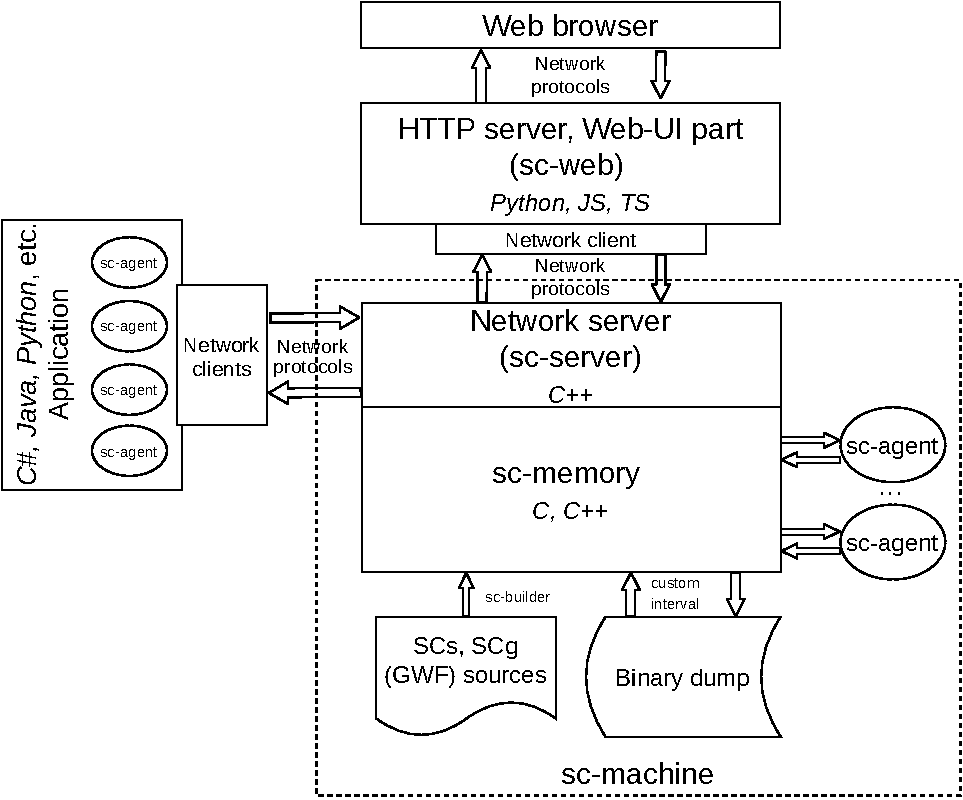
\includegraphics[scale=0.95]{figures/sd_interpreters/platform-ostis-architecture.pdf}}}
\scnaddlevel{1}
	\scnexplanation{На приведенной иллюстрации видно, что ядром платформы является \textit{Программная модель sc-памяти} (sc-machine), которая одновременно может взаимодействовать как с \textit{Реализацией интерпретатора sc-моделей пользовательских интерфейсов} (sc-web \scncite{sc_web}), так и с любыми сторонними приложениями по соответствующим сетевым протоколам. С точки зрения общей архитектуры \textit{Реализация интерпретатора sc-моделей пользовательских интерфейсов} выступает как один из множества возможных внешних компонентов, взаимодействующих с \textit{Программной моделью sc-памяти} по сети.}
\scnaddlevel{-1}

\scnheader{Программная модель sc-памяти}
\scnidtf{sc-machine}
\scnidtf{Программная модель семантической памяти, реализованная на основе традиционной линейной памяти и включающая средства хранения sc-конструкций и базовые средства для обработки этих конструкций, в том числе удаленного доступа к ним посредством соответствующих сетевых протоколов}
\scnrelto{программная модель}{sc-память}
\scniselement{программная модель sc-памяти на основе линейной памяти}
\scntext{основной репозиторий исходных текстов}{https://github.com/ostis-dev/sc-machine.git}
\scnrelfromlist{компонент программной системы}{Реализация sc-хранилища и средств доступа к нему\\
	\scnaddlevel{1}
		\scnexplanation{В рамках текущей \textit{Программной модели sc-памяти} под \textit{sc-хранилищем} понимается компонент программной модели, осуществляющий хранение sc-конструкций и доступ к ним через программный интерфейс. В общем случае \textit{sc-хранилище} может быть реализовано по-разному. Кроме собственно \textit{sc-хранилища} \scnbispace \textit{Программная модель sc-памяти} включает также \textit{Реализацию файловой памяти ostis-системы}, предназначенную для хранения содержимого \textit{внутренних файлов ostis-систем}. Стоит отметить, что при переходе с \textit{Программной модели sc-памяти} на ее аппаратную реализацию файловую память ostis-системы целесообразно будет реализовывать на основе традиционной линейной памяти (во всяком случае, на первых этапах развития \textit{семантического компьютера}).}
	\scnaddlevel{-1}
	;Реализация базового набора платформенно-зависимых sc-агентов и их общих компонентов;Реализация подсистемы взаимодействия с внешней средой с использованием сетевых протоколов;Реализация вспомогательных инструментальных средств для работы с sc-памятью;Реализация scp-интерпретатора}
\scntext{программная документация}{http://ostis-dev.github.io/sc-machine/}
\scnrelfromlist{используемый язык программирования}{C;C++;Python}
\scnnote{Текущий вариант \textit{Программной модели sc-памяти} предполагает возможность сохранения состояния (слепка) памяти на жесткий диск и последующей загрузки из ранее сохраненного состояния. Такая возможность необходима для перезапуска системы, в случае возможных сбоев, а также при работе с исходными текстами базы знаний, когда сборка из исходных текстов сводится к формированию слепка состояния памяти, который затем помещается в \textit{Программную модель sc-памяти}.}

\scnheader{Реализация sc-хранилища и средств доступа к нему}
\scnrelfromlist{компонент программной системы}{Реализация sc-хранилища;Реализация файловой памяти ostis-системы}

\scnheader{Реализация sc-хранилища}
\scniselement{реализация sc-хранилища на основе линейной памяти}
\scnrelfrom{иллюстрация}{\scnfileimage{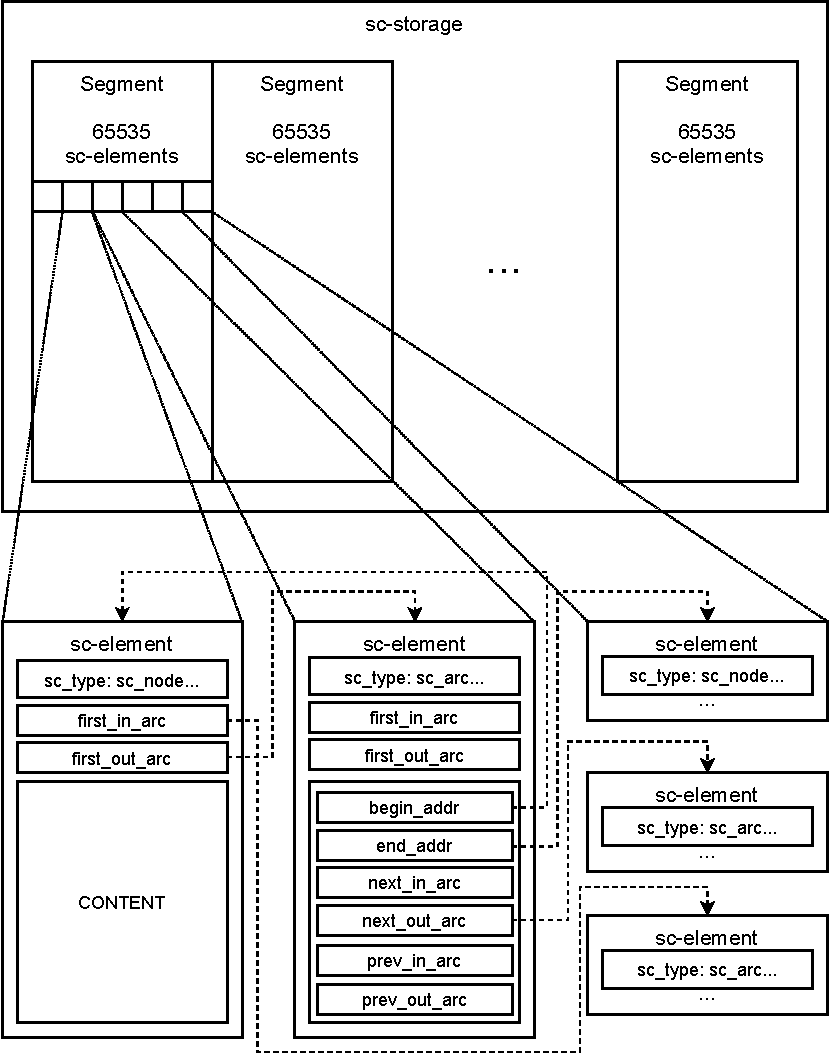
\includegraphics{figures/sd_interpreters/sc-storage.pdf}}}
\scnrelfrom{класс объектов программной системы}{сегмент sc-хранилища}
\scnaddlevel{1}
	\scnidtf{страница sc-хранилища}
	\scnexplanation{В рамках данной реализации \textit{sc-хранилища} \scnbigspace \textit{sc-память} моделируется в виде набора \textit{сегментов}, каждый из которых представляет собой фиксированного размера упорядоченную последовательность \textit{элементов sc-хранилища}, каждый из которых соответствует конкретному sc-элементу. В настоящее время каждый сегмент состоит из $2^{16}-1=65535$ \textit{элементов sc-хранилища}. Выделение \textit{сегментов sc-хранилища} позволяет, с одной стороны, упростить адресный доступ к \textit{элементам sc-хранилища}, с другой стороны -- реализовать возможность выгрузки части sc-памяти из оперативной памяти на файловую систему при необходимости. Во втором случае сегмент sc-хранилища становится минимальной (атомарной) выгружаемой частью sc-памяти. Механизм выгрузки сегментов реализуется в соответствии с существующими принципами организации виртуальной памяти в современных операционных системах.}
	\scnnote{Максимально возможное число сегментов ограничивается настройками программной реализации sc-хранилища (в настоящее время по умолчанию установлено количество $2^{16}-1=65535$ сегментов, но в общем случае оно может быть другим). Таким образом, технически максимальное количество хранимых sc-элементов в текущей реализации составляет около $4.3 \times 10^{9}$ sc-элементов.}
	\scnnote{По умолчанию все сегменты физически располагаются в оперативной памяти, если объема памяти не хватает, то предусмотрен механизм выгрузки части сегментов на жесткий диск (механизм виртуальной памяти).}
	\scnrelfrom{класс объектов программной системы}{элемент sc-хранилища}
		\scnaddlevel{1}
			\scnexplanation{Каждый сегмент состоит из набора структур данных, описывающих конкретные \textit{sc-элементы} (элементов sc-хранилища). Независимо от типа описываемого sc-элемента каждый \textit{элемент sc-хранилища} имеет фиксированный размер (в текущий момент -- 48 байт), что обеспечивает удобство их хранения. Таким образом, максимальный размер базы знаний в текущей программной модели sc-памяти может достигнуть 223 Гб (без учета содержимого \textit{внутренних файлов ostis-системы}, хранимого на внешней файловой системе).}
		\scnaddlevel{-1}
\scnaddlevel{-1}
\scnrelfrom{пример}{\scnfileimage{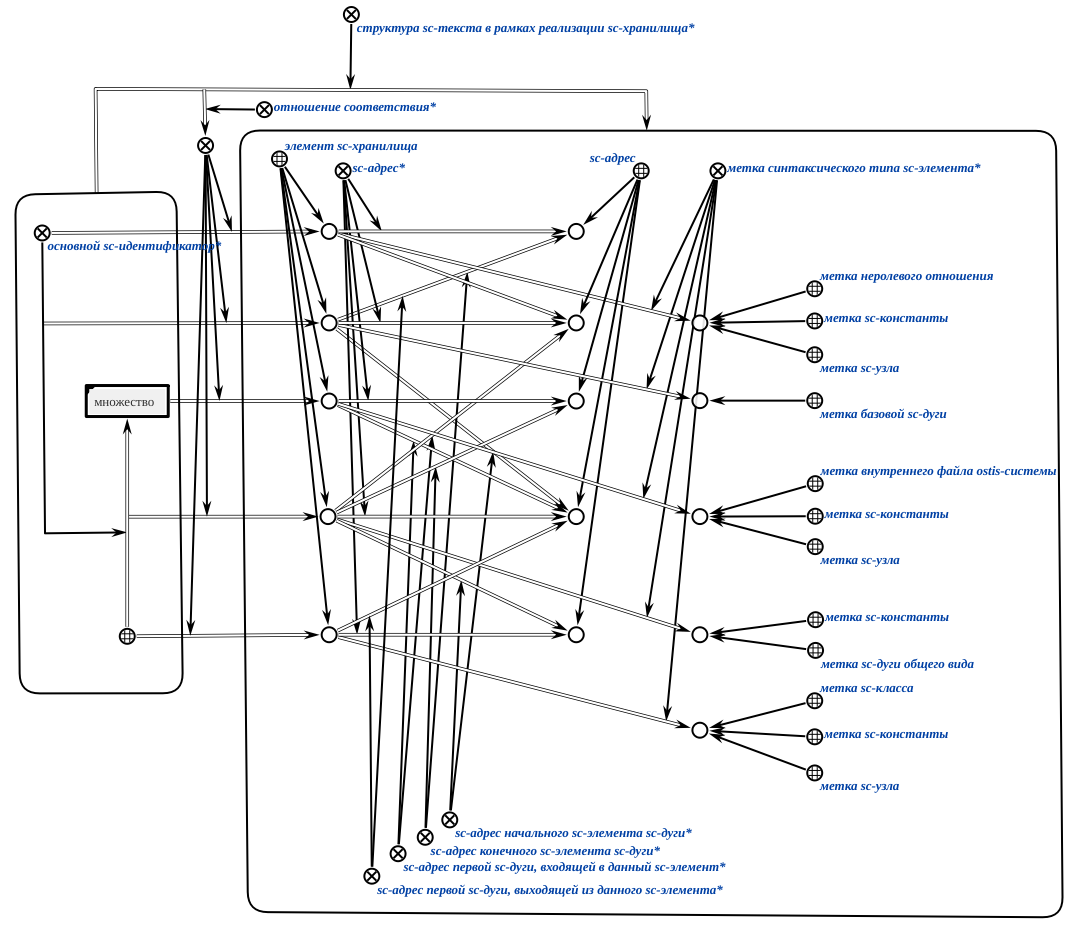
\includegraphics[scale=0.6]{figures/sd_interpreters/storage_example.png}}}
\scnaddlevel{1}
	\scnnote{Для наглядности в данном примере опущены \textit{метки уровня доступа}}
\scnaddlevel{-1}

\scnheader{sc-адрес}
\scnidtf{адрес элемента sc-хранилища, соответствующего заданному sc-элементу, в рамках текущего состояния реализации sc-хранилища в составе программной модели sc-памяти}
\scnexplanation{Каждый элемент sc-хранилища в текущей реализации может быть однозначно задан его адресом (sc-адресом), состоящим из номера сегмента и номера \textit{элемента sc-хранилища} в рамках сегмента. Таким образом, \textit{sc-адрес} служит уникальными координатами \textit{элемента sc-хранилища} в рамках \textit{Реализации sc-хранилища}.}
\scnnote{Sc-адрес никак не учитывается при обработке базы знаний на семантическом уровне и необходим только для обеспечения доступа к соответствующей структуре данных, хранящейся в линейной памяти на уровне \textit{Реализации sc-хранилища}.}
\scnnote{В общем случае sc-адрес элемента sc-хранилища, соответствующего заданному sc-элементу, может меняться, например, при пересборке базы знаний из исходных текстов и последующем перезапуске системы. При этом sc-адрес элемента sc-хранилища, соответствующего заданному sc-элементу, непосредственно в процессе работы системы в текущей реализации меняться не может.}
\scnnote{Для простоты будем говорить "sc-адрес sc-элемента"{}, имея в виду \textit{sc-адрес} \scnbigspace \textit{элемента sc-хранилища}, однозначно соответствующего данному \textit{sc-элементу}.}
\scnrelfromlist{семейство отношений, однозначно задающих структуру заданной сущности}{номер сегмента sc-хранилища*;номер элемента sc-хранилища в рамках сегмента*}

\scnheader{элемент sc-хранилища}
\scnidtf{ячейка sc-хранилища}
\scnidtf{элемент sc-хранилища, соответствующий sc-элементу}
\scnidtf{образ sc-элемента в рамках sc-хранилища}
\scnidtf{структура данных, каждый экземпляр которой соответствует одному sc-элементу в рамках sc-хранилища}
\scnexplanation{Каждый элемент sc-хранилища, соответствующий некоторому sc-элементу, описывается его синтаксическим типом (меткой), а также независимо от типа указывается sc-адрес первой входящей в данный sc-элемент sc-дуги и первой выходящей из данного sc-элемента sc-дуги (могут быть пустыми, если таких sc-дуг нет). 
	
Оставшиеся байты в зависимости от типа соответствующего sc-элемента (sc-узел или sc-дуга) могут использоваться либо для хранения содержимого внутреннего файла ostis-системы (может быть пустым, если sc-узел не является знаком файла), либо для хранения спецификации sc-дуги.}
\scnsubdividing{элемент sc-хранилища, соответствующий sc-узлу\\
	\scnaddlevel{1}
		\scnrelfromset{семейство отношений, однозначно задающих структуру заданной сущности}{метка синтаксического типа sc-элемента*;метка уровня доступа sc-элемента*;sc-адрес первой sc-дуги, выходящей из данного sc-элемента*;sc-адрес первой sc-дуги, входящей в данный sc-элемент*;содержимое элемента sc-хранилища*\\
		\scnaddlevel{1}
			\scnrelfrom{второй домен}{содержимое элемента sc-хранилища}
			\scnaddlevel{1}
				\scnidtf{содержимое элемента sc-хранилища, соответствующего внутреннему файлу ostis-системы}
			\scnaddlevel{-1}
			\scnexplanation{Каждый sc-узел в текущей реализации может иметь содержимое (может стать \textit{внутренним файлом ostis-системы}).
			В случае, если размер содержимого внутреннего файла ostis-системы не превышает 48 байт (размер \textit{спецификации sc-дуги в рамках sc-хранилища}, например небольшой \textit{строковый sc-идентификатор}), то это содержимое явно хранится в рамках элемента sc-хранилища в виде последовательности байт.
			В противном случае оно помещается в специальным образом организованную файловую память (за ее организацию отвечает отдельный модуль платформы, который в общем случае может быть устроен по-разному), а в рамках элемента sc-хранилища хранится уникальный адрес соответствующего файла, позволяющий быстро найти его на файловой системе.}
		\scnaddlevel{-1}}
		\scnaddlevel{1}
			\scnnote{\textit{sc-адрес первой sc-дуги, выходящей из данного sc-элемента*}, \textit{sc-адрес первой sc-дуги, входящей в данный sc-элемент*} и \textit{содержимое элемента sc-хранилища*} в общем случае могут отсутствовать (быть нулевыми, "пустыми"{}), но размер элемента в байтах останется тем же.}
		\scnaddlevel{-1}
	\scnaddlevel{-1}
	;элемент sc-хранилища, соответствующий sc-дуге\\
	\scnaddlevel{1}
	\scnrelfromset{семейство отношений, однозначно задающих структуру заданной сущности}{метка синтаксического типа sc-элемента*;метка уровня доступа sc-элемента*;sc-адрес первой sc-дуги, выходящей из данного sc-элемента*;sc-адрес первой sc-дуги, входящей в данный sc-элемент*;спецификация sc-дуги в рамках sc-хранилища*\\
		\scnaddlevel{1}
			\scnrelfrom{второй домен}{спецификация sc-дуги в рамках sc-хранилища}
			\scnaddlevel{1}
			\scnrelfromset{семейство отношений, однозначно задающих структуру заданной сущности}{sc-адрес начального sc-элемента sc-дуги*;sc-адрес конечного sc-элемента sc-дуги*;sc-адрес следующей sc-дуги, выходящей из того же sc-элемента*;sc-адрес следующей sc-дуги, входящей в тот же sc-элемент*;sc-адрес предыдущей sc-дуги, выходящей из того же sc-элемента*;sc-адрес предыдущей sc-дуги, входящей в тот же sc-элемент*}
			\scnaddlevel{-1}
		\scnaddlevel{-1}}
	\scnnote{sc-ребра в текущий момент хранятся так же, как sc-дуги, то есть имеют начальный и конечный sc-элементы, отличие заключается только в \textit{метке синтаксического типа sc-элемента}. Это приводит к ряду неудобств при обработке, но sc-ребра используются в настоящее время достаточно редко.}
	\scnaddlevel{-1}}
\scnaddlevel{1}
	\scnnote{С точки зрения программной реализации структура данных для хранения sc-узла и sc-остается остается та же, но в ней меняется список полей (компонентов).\\
	Кроме того, как можно заметить каждый элемент sc-хранилища (в том числе, \textit{элемент sc-хранилища, соответствующий sc-дуге}) не хранит список sc-адресов связанных с ним sc-элементов, а хранит sc-адреса одной выходящей и одной входящей дуги, каждая из которых в свою очередь хранит sc-адреса следующей и предыдущей дуг в списке исходящих и входящих sc-дуг для соответствующих элементов.\\
	Все перечисленное позволяет:
	\begin{scnitemize}	
		\item сделать размер такой структуры фиксированным (в настоящее время 48 байт) и не зависящим от синтаксического типа хранимого sc-элемента;
		\item обеспечить возможность работы с sc-элементами без учета их синтаксического типа в случаях, когда это необходимо (например, при реализации поисковых запросов вида ``Какие sc-элементы являются элементами данного множества'', ``Какие sc-элементы непосредственно связаны с данным sc-элементом'' и т.д.);
		\item обеспечить возможность доступа к \textit{элементу sc-хранилища} за константное время;
		\item обеспечить возможность помещения \textit{элемента sc-хранилища} в процессорный кэш, что в свою очередь, позволяет ускорить обработку sc-конструкций;
	\end{scnitemize}}
\scnaddlevel{-1}
\scnnote{Текущая \textit{Программная модель sc-памяти} предполагает, что вся sc-память физически расположена на одном компьютере. Для реализации распределенного варианта \textit{Программной модели sc-памяти} предполагается расширить \textit{sc-адрес} указанием адреса того физического устройства, где хранится соответствующий \textit{элемент sc-хранилища}.}

\scnheader{метка синтаксического типа sc-элемента}
\scnidtf{уникальный числовой идентификатор, однозначно соответствующий заданному типу sc-элементов и приписываемый соответствующему элементу sc-хранилища на уровне реализации}
\scnnote{Очевидно, что тип (класс, вид) sc-элемента в sc-памяти может быть задан путем явного указания принадлежности данного sc-элемента соответствующему классу (sc-узел, sc-дуга и т.д.).
	
Однако, в рамках \textit{платформы интерпретации sc-моделей компьютерных систем} должен существовать какой-либо набор \textit{меток синтаксического типа sc-элемента}, которые задают тип элемента на уровне платформы и не имеют соответствующей sc-дуги принадлежности (а точнее -- базовой sc-дуги), явно хранимой в рамках sc-памяти (ее наличие подразумевается, однако она не хранится явно, поскольку это приведет к бесконечному увеличению числа sc-элементов, которые необходимо хранить в sc-памяти). Как минимум, должна существовать метка, соответствующая классу \textit{базовая sc-дуга}, поскольку явное указание принадлежности sc-дуги данному классу порождает еще одну \textit{базовую sc-дугу}.

Таким образом, \textit{базовые sc-дуги}, обозначающие принадлежность sc-элементов некоторому известному ограниченному набору классов представлены \uline{неявно}. Этот факт необходимо учитывать в ряде случаев, например, при проверке принадлежности sc-элемента некоторому классу, при поиске всех выходящих sc-дуг из заданного sc-элемента и т.д.

При необходимости некоторые из таких неявно хранимых sc-дуг могут быть представлены явно, например, в случае, когда такую sc-дугу необходимо включить в какое-либо множество, то есть провести в нее другую sc-дугу. В этом случае возникает необходимость синхронизации изменений, связанных с данной sc-дугой (например, ее удалении), в явном и неявном ее представлении. В текущей \textit{Реализации sc-хранилища} данный механизм не реализован.

Таким образом, полностью отказаться от \textit{меток синтаксического типа sc-элементов} невозможно, однако увеличение их числа хоть и повышает производительность платформы за счет упрощений некоторых операций по проверке типов sc-элемента, но приводит к увеличению числа ситуаций, в которых необходимо учитывать явное и неявное представление sc-дуг, что, в свою очередь, усложняет развитие платформы и разработку программного кода для обработки хранимых sc-конструкций.}
\scnrelto{второй домен}{метка синтаксического типа sc-элемента*}
\scnsuperset{метка sc-узла}
\scnaddlevel{1}
	\scntext{числовое выражение в шестнадцатеричной системе}{0x1}
\scnaddlevel{-1}
\scnsuperset{метка внутреннего файла ostis-системы}
\scnaddlevel{1}
\scntext{числовое выражение в шестнадцатеричной системе}{0x2}
\scnaddlevel{-1}
\scnsuperset{метка sc-ребра общего вида}
\scnaddlevel{1}
\scntext{числовое выражение в шестнадцатеричной системе}{0x4}
\scnaddlevel{-1}
\scnsuperset{метка sc-дуги общего вида}
\scnaddlevel{1}
\scntext{числовое выражение в шестнадцатеричной системе}{0x8}
\scnaddlevel{-1}
\scnsuperset{метка sc-дуги принадлежности}
\scnaddlevel{1}
\scntext{числовое выражение в шестнадцатеричной системе}{0x10}
\scnaddlevel{-1}
\scnsuperset{метка sc-константы}
\scnaddlevel{1}
\scntext{числовое выражение в шестнадцатеричной системе}{0x20}
\scnaddlevel{-1}
\scnsuperset{метка sc-переменной}
\scnaddlevel{1}
\scntext{числовое выражение в шестнадцатеричной системе}{0x40}
\scnaddlevel{-1}
\scnsuperset{метка позитивной sc-дуги принадлежности}
\scnaddlevel{1}
\scntext{числовое выражение в шестнадцатеричной системе}{0x80}
\scnaddlevel{-1}
\scnsuperset{метка негативной sc-дуги принадлежности}
\scnaddlevel{1}
\scntext{числовое выражение в шестнадцатеричной системе}{0x100}
\scnaddlevel{-1}
\scnsuperset{метка нечеткой sc-дуги принадлежности}
\scnaddlevel{1}
\scntext{числовое выражение в шестнадцатеричной системе}{0x200}
\scnaddlevel{-1}
\scnsuperset{метка постоянной sc-дуги}
\scnaddlevel{1}
\scntext{числовое выражение в шестнадцатеричной системе}{0x400}
\scnaddlevel{-1}
\scnsuperset{метка временной sc-дуги}
\scnaddlevel{1}
\scntext{числовое выражение в шестнадцатеричной системе}{0x800}
\scnaddlevel{-1}
\scnsuperset{метка небинарной sc-связки}
\scnaddlevel{1}
\scntext{числовое выражение в шестнадцатеричной системе}{0x80}
\scnaddlevel{-1}
\scnsuperset{метка sc-структуры}
\scnaddlevel{1}
\scntext{числовое выражение в шестнадцатеричной системе}{0x100}
\scnaddlevel{-1}
\scnsuperset{метка ролевого отношения}
\scnaddlevel{1}
\scntext{числовое выражение в шестнадцатеричной системе}{0x200}
\scnaddlevel{-1}
\scnsuperset{метка неролевого отношения}
\scnaddlevel{1}
\scntext{числовое выражение в шестнадцатеричной системе}{0x400}
\scnaddlevel{-1}
\scnsuperset{метка sc-класса}
\scnaddlevel{1}
\scntext{числовое выражение в шестнадцатеричной системе}{0x800}
\scnaddlevel{-1}
\scnsuperset{метка абстрактной сущности}
\scnaddlevel{1}
\scntext{числовое выражение в шестнадцатеричной системе}{0x1000}
\scnaddlevel{-1}
\scnsuperset{метка материальной сущности}
\scnaddlevel{1}
\scntext{числовое выражение в шестнадцатеричной системе}{0x2000}
\scnaddlevel{-1}
\scnsuperset{метка константной позитивной постоянной sc-дуги принадлежности}
\scnaddlevel{1}
\scnidtf{метка базовой sc-дуги}
\scnidtf{метка sc-дуги основного вида}
\scnreltoset{пересечение}{метка sc-дуги принадлежности;метка sc-константы;метка позитивной sc-дуги принадлежности;метка постоянной sc-дуги}
\scnnote{\textit{метки синтаксических типов sc-элементов} могут комбинироваться между собой для получения более частных классов меток. С точки зрения программной реализации такая комбинация выражается операцией побитового сложения значений соответствующих меток.}
\scnaddlevel{-1}
\scnsuperset{метка переменной позитивной постоянной sc-дуги принадлежности}
\scnaddlevel{1}
\scnreltoset{пересечение}{метка sc-дуги принадлежности;метка sc-переменной;метка позитивной sc-дуги принадлежности;метка постоянной sc-дуги}
\scnaddlevel{-1}
\scnnote{Числовые выражения некоторых классов меток могут совпадать. Это сделано для уменьшения размера элемента sc-хранилища за счет уменьшения максимального размера метки. Конфликт в данном случае не возникает, поскольку такие классы меток не могут комбинироваться, например \textit{метка ролевого отношения} и \textit{метка нечеткой sc-дуги принадлежности}.}
\scnnote{Важно отметить, что каждому из выделенных классов меток (кроме классов, получаемых путем комбинации других классов) однозначно соответствует порядковый номер бита в линейной памяти, что можно заметить, глядя на соответствующие числовые выражения классов меток. Это означает, что классы меток не включаются друг в друга, например, указание \textit{метки позитивной sc-дуги принадлежности} не означает автоматическое указание \textit{метки sc-дуги принадлежности}. Это позволяет сделать операции комбинирования и сравнения меток более эффективными.}
\scnreltoset{недостатки текущего состояния}{
\scnfileitem{На данный момент число \textit{меток синтаксического типа sc-элемента} достаточно велико, что приводит к возникновению достаточно большого числа ситуаций, в которых нужно учитывать явное и неявное хранение sc-дуг принадлежности соответствующим классам. С другой стороны, изменение набора меток с какой-либо целью в текущем варианте реализации представляет собой достаточно трудоемкую задачу (с точки зрения объема изменений в программном коде платформы и sc-агентов, реализованных на уровне платформы), а расширение набора меток без увеличения объема элемента sc-хранилища в байтах оказывается и вовсе невозможным.}\\
	\scnaddlevel{1}
		\scntext{вариант решения}{Решением данной проблемы является максимально возможная минимизация числа меток, например, до числа меток, соответствующих \textit{Алфавиту SC-кода}. В таком случае принадлежность sc-элементов любым другим классам будет записываться явно, а число ситуаций, в которых необходимо будет учитывать неявное хранение sc-дуг, будет минимальным.}
	\scnaddlevel{-1}
;
\scnfileitem{Некоторые метки из текущего набора \textit{меток синтаксического типа sc-элемента} используются достаточно редко (например, \textit{метка sc-ребра общего вида} или \textit{метка негативной sc-дуги принадлежности}), в свою очередь, в sc-памяти могут существовать классы, имеющие достаточно много элементов (например, \textit{бинарное отношение} или \textit{число}). Данный факт не позволяет в полной мере использовать эффективность наличия меток.}
	\scnaddlevel{1}
		\scntext{вариант решения}{Решением данной проблемы является отказ от заранее известного набора меток и переход к динамическому набору меток (при этом их число может оставаться фиксированным). В этом случае набор классов, выражаемых в виде меток будет формироваться на основании каких-либо критериев, например, числа элементов данного класса или частоты обращений к нему.}
	\scnaddlevel{-1}
}

\scnheader{метка уровня доступа sc-элемента}
\scnrelto{второй домен}{метка уровня доступа sc-элемента*}
\scnrelfromset{обобщенная структура}{метка уровня доступа sc-элемента на чтение;метка уровня доступа sc-элемента на запись}
\scnexplanation{В текущей \textit{Реализации sc-хранилища} \scnbigspace \textit{метки уровня доступа} используются для того, чтобы обеспечить возможность ограничения доутспа некоторых процессов в sc-памяти к некоторым sc-элементам, хранимым в sc-памяти.
	
Каждому элементу sc-хранилища соответствует \textit{метка уровня доступа sc-элемента на чтение} и \textit{метка уровня доступа sc-элемента на запись}, каждая из которых выражается числом от 0 до 255. 
	
В свою очередь, каждому процессу (чаще всего, соответствующему некоторому sc-агенту), который пытается получить доступ к данному элементу sc-хранилища (прочитать или изменить его) соответствует уровень доступа на чтение и запись, выраженный в том же числовом диапазоне. Указанный уровень доступа для процесса является частью \textit{контекста процесса}. Доступ на чтение или запись к элементу sc-хранилища не разрешается, если уровень доступа соответственно на чтение или запись у процесса ниже, чем у элемента sc-хранилища, к которому осуществляется доступ.

Таким образом нулевое значение \textit{метки уровня доступа sc-элемента на чтение} и \textit{метки уровня доступа sc-элемента на запись} означает, что любой процесс может получить неограниченный доступ к данному элементу sc-хранилища.}

\scnheader{sc-итератор}
\scnidtf{ScIterator}
\scnrelto{класс компонентов}{Реализация sc-хранилища}
\scnexplanation{С функциональной точки зрения \textit{sc-итераторы} как часть \textit{Реализации sc-хранилища} представляют собой базовое средство доступа к конструкциям, хранимым в sc-памяти, которое позволяет осуществить чтение (просмотр) конструкций, изоморфных простейшим шаблонам -- \textit{трехэлементным sc-конструкциям} и \textit{пятиэлементным sc-конструкциям} (см. \textit{Раздел \nameref{sec:sd_ps}}).
	
С точки зрения реализации \textit{sc-итератор} представляет собой структуру данных, которая соответствует определенному дополнительно уточняемому классу sc-конструкций и позволяет при помощи соответствующего набора функций последовательно осуществлять просмотр всех sc-конструкций данного класса, представленных в текущем состоянии sc-памяти (итерацию по sc-конструкциям).
	
Каждому классу \textit{sc-итераторов} соответствует некоторый известный класс (шаблон, образец) sc-конструкций. При создании sc-итератора данный шаблон уточняется, то есть некоторым (как минимум одному) элементам шаблона ставится в соответствие конкретный заранее известный \textit{sc-элемент} (отправная точка при поиске), а другим элементам шаблона (тем, которые нужно найти) ставится в соответствие некоторый тип sc-элемента из числа типов, соответствующих \textit{меткам синтаксического типа sc-элемента}. 

Далее путем вызова соответствующей функции (или метода класса в ООП) осуществляется последовательный просмотр всех sc-конструкций, соответствующих полученному шаблону (с учетом указанных типов sc-элементов и заранее заданных известных sc-элементов), то есть \textit{sc-итератор} последовательно "переключается"{} с одной конструкции на другую до тех пор, пока такие конструкции существуют. Проверка существования следующей конструкции проверяется непосредственно перед переключением. В общем случае конструкций, соответствующих указанному шаблону, может не существовать, в этом случае итерирование происходить не будет (будет 0 итераций).

На каждой итерации в sc-итератор записываются sc-адреса sc-элементов, входящих в соответствующую sc-конструкцию, таким образом найденные элементы могут быть обработаны нужным образом в зависимости от задачи.}
\scnsuperset{трехэлементный sc-итератор}
	\scnaddlevel{1}
		\scnrelfrom{класс sc-конструкций}{трехэлементная sc-конструкция}
	\scnaddlevel{-1}
\scnsuperset{пятиэлементный sc-итератор}
	\scnaddlevel{1}
		\scnrelfrom{класс sc-конструкций}{пятиэлементная sc-конструкция}
		\scnnote{В настоящее время \textit{пятиэлементный sc-итератор} реализуется на основе \textit{трехэлементных sc-итераторов} и в этом смысле не является атомарным. Однако, введение \textit{пятиэлементных sc-итераторов} целесообразно с точки зрения удобства разработчика программ обработки sc-конструкций.}
	\scnaddlevel{-1}

\scnheader{sc-шаблон}
\scnidtf{ScTemplate}
\scnidtf{структура данных в линейной памяти, описывающая обобщенную sc-структуру, которая в свою очередь может быть либо явно представлена sc-памяти, либо не представлена в ее текущем состоянии, но может быть представлена при необходимости}
\scnrelto{класс компонентов}{Реализация sc-хранилища}
\scnexplanation{\textit{Sc-итераторы} позволяют осуществлять поиск только sc-конструкций простейшей конфигурации. Для реализации поиска sc-конструкций более сложной конфигурации, а также генерации сложных sc-конструкций используются \textit{sc-шаблоны}, на основе которых затем осуществляется поиск или генерация конструкций. \textit{Sc-шаблон} представляет собой структуру данных, соответствующую некоторой \textit{обобщенной sc-структуре}, т.е. \textit{sc-структуре}, содержащей \textit{sc-переменные}. При помощи соответствующего набора функций можно осуществлять 
\begin{scnitemize}
	\item поиск в текущем состоянии sc-памяти \uline{всех} sc-конструкций, изоморфных заданному шаблону. В качестве параметров поиска можно указать значения для каких-либо из sc-переменных в составе шаблона. После осуществления поиска будет сформировано множество результатов поиска, каждый из которых представляет собой множество пар вида ``sc-переменная из шаблона -- соответствующая ей sc-константа''. Данное множество может быть пустым (в текущем состоянии sc-памяти нет конструкций, изоморфных заданному образцу) или содержать один или более элементов. Подстановка значений sc-переменных может осуществляться как по sc-адресу, так и по системному sc-идентификатору;
	\item генерацию sc-конструкции, изоморфной заданному шаблону. Параметры и результаты генерации формируются так же, как в случае поиска, за исключением того, что в случае генерации результат всегда один и множество результатов не формируется;
\end{scnitemize}

Таким образом, каждый \textit{sc-шаблон} фактически задает множество шаблонов, формируемых путем указания значений для sc-переменных, входящих в исходный шаблон.

Важно отметить, что \textit{sc-шаблон} представляет собой структуру данных в линейной памяти, соответствующую некоторой \textit{обобщенной sc-структуре} в sc-памяти, но не саму эту \textit{обобщенную sc-структуру}. Это означает, что sc-шаблон может быть автоматически сформирован на основе \textit{обобщенной sc-структуры}, явно представленной в sc-памяти, а также сформирован на уровне программного кода путем вызова соответствующих функций (методов). Во втором случае \textit{sc-шаблон} будет существовать только в линейной памяти и соответствующая \textit{обобщенная sc-структура} не будет явно представлена в sc-памяти. В этом случае подстановка значений sc-переменных будет возможна только по системному sc-идентификатору, поскольку sc-адресов у соответствующих элементов шаблона существовать не будет.}
\scnnote{При поиске sc-конструкций, изоморфных заданному шаблону, крайне важно с точки зрения производительности с какого sc-элемента начинать поиск. Как известно, в общем случае задача поиска в графе представляет собой NP-полную задачу, однако поиск в sc-графе позволяет учитывать семантику обрабатываемой информации, что, в свою очередь, позволяет существенно снизить время поиска. 
	
Одним из возможных вариантов оптимизации алгоритма поиска, реализованным на данный момент, является упорядочение трехэлементных sc-конструкций, входящих в состав sc-шаблона, по очередности поиска по этим sc-конструкциям по критерию снижения числа возможных вариантов поиска, которые порождает та или иная трехэлементная sc-конструкция, содержащая sc-переменные. Так, в первую очередь при поиске выбираются те трехэлементные sc-конструкции, которые изначально содержат две sc-константы, затем те, которые изначально содержат одну sc-константу. После выполнения шага поиска приоритет sc-конструкций изменяется с учетом результатов, полученных на предыдущем шаге.

Другой вариант оптимизации основывается на той особенности формализации в SC-коде, что в общем случае число sc-дуг, входящих в некоторый sc-элемент, как правило значительно меньше числа выходящих из него sc-дуг. Таким образом, целесообразным оказывается осуществлять поиск вначале по входящим sc-дугам.}
\scnnote{Можно предположить, что возможности, предоставляемые \textit{sc-шаблонами} позволяют полностью исключить использование \textit{sc-итераторов}. Однако это не совсем так по следующим причинам:
	\begin{scnitemize}
		\item функции поиска и генерации по шаблону реализуются на основе sc-итераторов, как базового средства поиска sc-конструкций в рамках \textit{Реализации sc-хранилища}.
		\item \textit{sc-итераторы} дают возможность более гибко организовать процесс поиска с учетом семантики конкретных sc-элементов, участвующих в поиске. Так например, можно учесть тот факт, что для некоторых sc-элементов число входящих sc-дуг значительно меньше, чем выходящих (или наоборот) таким образом, при поиске конструкций, содержащих такие sc-элементы более эффективно начать перебор с тех участков, где дуг потенциально меньше.
\end{scnitemize}}

\scnheader{контекст процесса в рамках программной модели sc-памяти}
\scnidtf{ScContext}
\scnidtf{контекст процесса, выполняемого на уровне программной модели sc-памяти}
\scnidtf{метаописание процесса в sc-памяти, выполняемого на уровне программной модели sc-памяти}
\scnidtf{структура данных, содержащая метаинформацию о процессе, выполняемом в sc-памяти на уровне платформы}
\scnrelto{класс компонентов}{Реализация sc-хранилища}
\scnexplanation{Каждому процессу, выполняемому в sc-памяти на уровне \textit{платформы интерпретации sc-моделей компьютерных систем} (и чаще всего соответствующего некоторому \textit{sc-агенту}, реализованному на уровне платформы) ставится в соответствие \textit{контекст процесса}, который является структурой данных, описывающей метаинформацию о данном процессе. На текущий момент контекст процесса содержит сведения об уровне доступа на чтение и запись для данного процесса (См. \textit{метка уровня доступа sc-элемента}).

При вызове в рамках процесса любых функций (методов), связанных с доступом к хранимым в sc-памяти конструкциям одним из параметров обязательно является \textit{контекст процесса}.}

\scnheader{блокировка sc-элемента в рамках программной модели sc-памяти}
\scnidtf{ScLock}
\scnrelto{класс компонентов}{Реализация sc-хранилища}
\scnrelfrom{смотрите}{\nameref{sec:sd_agents}}

\scnheader{подписка на событие в sc-памяти в рамках программной модели sc-памяти}
\scnidtf{ScEvent}
\scnidtf{структура данных, описывающая в рамках программной модели sc-памяти соответствие между классом событий в sc-памяти и действиями, которые должно быть совершены при возникновении в sc-памяти событий данного класса}
\scnrelto{класс компонентов}{Реализация sc-хранилища}
\scnexplanation{Для того, чтобы обеспечить возможность создания sc-агентов в рамках \textit{платформы интерпретации sc-моделей компьютерных систем} реализована возможность создать подписку на событие, принадлежащее одному из классов \textit{элементарных событий в sc-памяти*} (см. Раздел ``\textit{Предметная область и онтология темпоральных сущностей базы знаний ostis-системы}''), уточнив при этом sc-элемент, с которым должно быть связано событие данного класса (например, sc-элемент, для которого должна появиться входящая или исходящая sc-дуга). Подписка на событие представляет собой структуру данных, описывающую класс ожидаемых событий и функцию в программном коде, которая должна быть вызвана при возникновении данного события.
	
Все подписки на события регистрируются в рамках таблицы событий. При любом изменении в sc-памяти происходит просмотр данной таблицы и запуск функций, соответствующих произошедшему событию.

В текущей реализации обработка каждого события осуществляется в отдельном потоке операционной системы, при этом на уровне реализации задается параметр, описывающий число максимальных потоков, которые могут выполняться параллельно.

Таким образом оказывается возможным реализовать sc-агенты, реагирующие на события в sc-памяти, а также при выполнении некоторого процесса в sc-памяти приостановить его работу и дождаться возникновения некоторого события (например, создать подзадачу некоторому коллективу sc-агентов и дождаться ее решения).}

\scnheader{Реализация файловой памяти ostis-системы}
\scnexplanation{Для хранения содержимого внутренних файлов ostis-систем, размер которого превышает 48 байт, используются файлы, явно хранимые на файловой системе, доступ к которой осуществляется средствами операционной системы, на которой работает \textit{Программный вариант реализации платформы интерпретации sc-моделей компьютерных систем}.

В общем случае множество различных внутренних файлов ostis-системы могут иметь одинаковое содержимое. Было бы разумно не хранить содержимое одинаковых файлов дважды. Для этого при создании соответствуюещго sc-узла и указании файла на файловой системе, который является содержимым данного sc-узла, вычисляется hash-сумма содержимого с помощью алгоритма SHA256. В результате получается строка из 32 символов, которая и выступает в качестве \textit{содержимого элемента sc-хранилища*}. Само же содержимое копируется в
файл на файловой системе, путь к которому строится на основании hash-суммы. Рядом с этим файлом создается файл, в котором хранятся sc-адреса всех sc-узлов, имеющих одно и то же ранее указанное содержимое. Таким образом, для того, чтобы найти все sc-узлы, имеющие указанное содержимое, необходимо вычислить hash-сумму искомого содержимого-образца и проверить наличие файла на файловой системе по пути, вычисляемому из hash-суммы и если он существует, то вернуть список хранящихся sc-адресов.

Кроме того, для реализации быстрого поиска sc-элементов по их строковым sc-идентификаторам или их фрагментам (подстрокам) используется дополнительное хранилище вида ключ-значение, которое ставит в соответствие \textit{строковому sc-идентификатору} \scnbigspace \textit{sc-адрес} того \textit{sc-элемента}, идентификатором которого является данная строка (в случае основного и системного sc-идентификатора) или \textit{sc-элемента}, который является знаком \textit{внутреннего файла ostis-системы} (в случае неосновного sc-идентификатора).}

\scnheader{Реализация базового набора платформенно-зависимых sc-агентов и их общих компонентов}
\scnidtf{sc-kpm}
\scnrelfromlist{компонент программной системы}{Реализация базового набора поисковых sc-агентов\\
	\scnaddlevel{1}
		\scnrelfromlist{используемый язык программирования}{C}
		\scnrelfromlist{компонент программной системы}{Реализация Абстрактного sc-агента поиска семантической окрестности заданной сущности;Реализация Абстрактного sc-агента поиска всех сущностей, частных по отношению к заданной;Реализация Абстрактного sc-агента поиска всех сущностей, общих по отношению к заданной;Реализация Абстрактного sc-агента поиска всех sc-идентификаторов, соответствующих заданной сущности;Реализация Абстрактного sc-агента поиска базовых sc-дуг, инцидентных заданному sc-элементу\\
			\scnaddlevel{1}
				\scnrelfromlist{компонент программной системы}{Реализация Абстрактного sc-агента поиска базовых sc-дуг, входящих в заданный sc-элемент;Реализация Абстрактного sc-агента поиска базовых sc-дуг, выходящих из заданного sc-элемента;Реализация Абстрактного sc-агента поиска базовых sc-дуг, входящих в заданный sc-элемент, с указанием множеств, которым принадлежат эти sc-дуги;Реализация Абстрактного sc-агента поиска базовых sc-дуг, выходящих из заданного sc-элемента, с указанием множеств, которым принадлежат эти sc-дуги}
			\scnaddlevel{-1}}
	\scnaddlevel{-1}
	;Реализация базового механизма сборки информационного мусора\\
	\scnaddlevel{1}
		\scnrelfromlist{используемый язык программирования}{C}	
		\scnnote{Текущая реализация механизма сборки информационного мусора содержит один sc-агент, реагирующий на явное добавление какого-либо sc-элемента во множество ``информационный мусор'' и осуществляющий физическое удаление этого sc-элемента из sc-памяти}
	\scnaddlevel{-1}
	;Реализация базового набора интерфейсных sc-агентов\\
	\scnaddlevel{1}
	\scnrelfromlist{используемый язык программирования}{C++}	
	\scnrelfromlist{компонент программной системы}{Реализация Абстрактного sc-агента обработки команд пользовательского интерфейса;Реализация Абстрактного sc-агента трансляции из внутреннего представления знаний во промежуточный транспортный формат\\
	\scnaddlevel{1}
		\scnnote{В настоящее время используется подход, при котором независимо от формы внешнего представления информации, информация хранимая в sc-памяти вначале транслируется в промежуточный транспортный формат на базе JSON, который затем обрабатывается sc-агентами пользовательского интерфейса, входящими в состав \textit{Реализации интерпретатора sc-моделей пользовательских интерфейсов}}
	\scnaddlevel{1}
	}
	\scnaddlevel{-1}
}

\scnheader{Реализация подсистемы взаимодействия с внешней средой с использованием сетевых протоколов}
\scnrelfromlist{компонент программной системы}{Реализация подсистемы взаимодействия с внешней средой с использованием протокола SCTP;Реализация подсистемы взаимодействия с внешней средой с использованием протоколов на основе формата JSON}
\scnexplanation{Взаимодействие программной модели sc-памяти с внешними ресурсами может осуществляться посредством специализированного программного интерфейса (API), однако этот вариант неудобен в большинстве случае, поскольку:
	\begin{scnitemize}
		\item поддерживается только для очень ограниченного набора языков программирования (С, С++, Python);
		\item требует того, чтобы клиентское приложение, обращающееся к программной модели sc-памяти, фактически составляло с ней единое целое, таким образом исключается возможность построения распределенного коллектива ostis-систем;
		\item как следствие предыдущего пункта, исключается возможность параллельной работы с sc-памятью нескольких клиентских приложений.
	\end{scnitemize}
	
Для того, чтобы обеспечить возможность удаленного доступа к sc-памяти не учитывая при этом языки программирования, с помощью которых реализовано конкретное клиентское приложение, было принято решение о реализации возможности доступа к sc-памяти с использованием универсальных протоколов, не зависящих от средств реализации того или иного компонента или системы. В качестве таких протоколов были разработаны бинарный протокол SCTP и текстовый протокол на базе JSON.}

\scnheader{SCTP}
\scnidtf{Semantic Code Transfer Protocol}
\scnrelboth{аналогия}{HTTP}
\scnexplanation{SCTP представляет собой \textit{бинарный протокол}, позволяющий осуществлять операции чтения (поиска) и редактирования конструкций, хранящихся в sc-памяти, а также отслеживать события, происходящие в sc-памяти.

Взаимодействие между клиентом и сервером на протоколе SCTP осуществляется путем обмена \textit{sctp-командами}, каждая из которых представляет собой набор байт, предназначенный для машинной обработки (но не восприятия человеком).
}

\scnheader{следует отличать*}
\scnhaselementset{SCTP\\
	\scnaddlevel{1}
	\scnidtf{Semantic Code Transfer Protocol}
	\scnaddlevel{-1};
	Stream Control Transmission Protocol\\
	\scnaddlevel{1}
	\scnidtf{Протокол передачи с управлением потоком}
	\scnnote{Протокол транспортного уровня в компьютерных сетях, разработанный в 2000 году.}
	\scnaddlevel{-1}}

\scnheader{sctp-команда}
\scnrelfromset{обобщенная декомпозиция}{заголовок sctp-команды\\
	\scnaddlevel{1}
		\scnidtf{часть sctp-команды, в которой указан её тип и некоторая дополнительная информация о ней}
	\scnaddlevel{-1}
	;аргументы sctp-команды\\
	\scnaddlevel{1}
		\scnidtf{часть sctp-команды, которая содержит её аргументы и размер которой может быть разным в зависимости от типа команды.}
	\scnaddlevel{-1}}
\scnrelfromlist{включение;пример}{sctp-команда удаления sc-элемента с указанным sc-адресом;sctp-команда создания нового sc-узла указанного типа;sctp-команда получения начального и конечного элемента sc-дуги}
\scnnote{Выполнение каждой sctp-команды предполагает наличие sctp-результата, однозначно соответствующего данной команде.}

\scnheader{SCTP}
\scntext{программная документация}{http://ostis-dev.github.io/sc-machine/net/sctp/}
\scnrelfromlist{недостаток}{\scnfileitem{Команды протокола SCTP являются низкоуровневыми (ориентированы на работу с единичными sc-элементами или простейшими sc-конструкциями из 3 или 5 элементов). Это приводит к тому, что выполнение даже несложного преобразования в базе знаний или ассоциативный поиск по набору взаимосвязанных конструкций выражаются в виде достаточно большого набора sctp-команд. С учетом того, что для каждой команды существует sctp-результат, также пересылаемый по сети, это излишне нагружает сеть и сильно ухудшает производительность системы в целом. Кроме того, производительность системы начинает сильно зависеть от пропускной способности сети.};
\scnfileitem{Протокол SCTP не предназначен для восприятия человеком}}
\scnrelfromlist{достоинство}{\scnfileitem{Протокол SCTP является кросс-платформенным};\scnfileitem{Протокол SCTP может быть достаточно просто реализован практически на любом языке программирования}}
\scnrelfromlist{обобщенная реализация}{sctp-сервер\\
	\scnaddlevel{1}
		\scnexplanation{Sctp-сервер обрабатывает sctp-команды, приходящие от разных sctp-клиентов, и обеспечивает их интерпретацию в sc-памяти.}
	\scnaddlevel{-1}
	;sctp-клиент\\
	\scnaddlevel{1}
		\scnexplanation{Sctp-клиенты в общем случае могут быть реализованы на разных языках программирования и иметь разный программный интерфейс. По сути задачей sctp-клиента является преобразование высокоуровневых команд представленных в форме, удобной программисту, в одну или более низкоуровневых sctp-команд, отправка их на сервер, ожидание sctp-результата и его интерпретация.}
	\scnaddlevel{-1}}

\scnheader{Реализация подсистемы взаимодействия с внешней средой с использованием протокола SCTP}
\scnrelfromlist{компонент программной системы}{Реализация sctp-сервера;Реализация sctp-клиента\\
	\scnaddlevel{1}
	\scnnote{\textit{Реализация подсистемы взаимодействия с внешней средой с использованием протокола SCTP} включает в себя \textit{Реализацию sctp-клиента} на языке C++, в то же время есть другие реализации \textit{sctp-клиентов} в рамках того же программного варианта реализации платформы, например, в рамках \textit{Реализации интерпретатора sc-моделей пользовательских интерфейсов}.}
	\scnaddlevel{-1}}

\scnheader{Реализация подсистемы взаимодействия с внешней средой с использованием протоколов на основе формата JSON}
\scnexplanation{В связи с большим числом недостатков протокола SCTP было принято решение о разработке другого протокола на основе какого-либо общепринятого текстового транспортного формата. В качестве такого формата был выбран формат JSON.}
\scnrelto{реализация}{Протокол взаимодействия с sc-памятью на основе JSON}
\scnaddlevel{1}
\scnnote{Данный протокол пока не имеет собственного названия}
\scntext{программная документация}{http://ostis-dev.github.io/sc-machine/http/websocket/}
\scnexplanation{В рамках \textit{Протокола взаимодействия с sc-памятью на основе JSON} каждая команда представляет собой json-объект, в котором указываются идентификатор команда, тип команды и ее аргументы. В свою очередь ответ на команду также представляет собой json-объект, в котором указываются идентификатор команды, ее статус (выполнена успешно/безуспешно) и результаты. Структура аргументов и результатов команды определяется типом команды.}
\scnrelfromlist{достоинство}{\scnfileitem{JSON является общепринятым открытым форматом, для работы с которым существует большое количество библиотек для популярных языков программирования. Это, в свою очередь, упрощает реализацию клиента и сервера для протокола, построенного на базе JSON.};
\scnfileitem{Реализация протокола на базе JSON не накладывает принципиальных ограничений на объем (длину) каждой команды, в отличие от бинарного протокола. Таким образом, появляется возможность использования неатомарных команд, позволяющих, например, за один акт пересылки такой команды по сети создать сразу несколько sc-элементов. Важными примерами таких команд являются  \textit{Команда генерации по произвольному образцу} и \textit{Команда поиска по произвольному образцу}.}}
\scnnote{Можно сказать, что протокол на базе JSON является следующим шагом на пути к созданию мощного и универсального языка запросов, аналогичного языку SQL для реляционных баз данных и предназначенному для работы с sc-памятью. Следующий шагом станет реализация такого протокола на основе одного из стандартов внешнего отображения sc-конструкций, например, \textit{SCs-кода}, что, в свою очередь, позволит передавать в качестве команд целые программы обработки sc-конструкций, например на языке SCP.}
\scnaddlevel{-1}

\scnheader{Реализация вспомогательных инструментальных средств для работы с sc-памятью}
\scnrelfrom{компонент программной системы}{Реализация сборщика базы знаний из исходных текстов, записанных в SCs-коде}
\scnaddlevel{1}
\scnidtf{sc-builder}
\scnrelfrom{используемый язык}{SCs-код}
\scnexplanation{Сборщик базы знаний из исходных текстов позволяет осуществить сборку базы знаний из набора исходных текстов, записанных в SCs-коде с ограничениями (см. \textit{Раздел **про исходные тексты**}) в бинарный формат, воспринимаемый \textit{Программной моделью sc-памяти}. При этом возможна как сборка "с нуля"{} (с уничтожением ранее созданного слепка памяти), так и аддитивная сборка, когда информация, содержащаяся в заданном множестве файлов, добавляется к уже имеющемуся слепку состояния памяти.

В текущей реализации сборщик осуществляет "склеивание"{} ("слияние"{}) sc-элементов, имеющих на уровне исходных текстов одинаковые \textit{системные sc-идентификаторы}.}
\scnaddlevel{-1}

\scnheader{Реализация интерпретатора sc-моделей пользовательских интерфейсов}
\scnidtf{sc-web}
\scnexplanation{Наряду с реализацией \textit{Программной модели sc-памяти} важной частью \textit{Программного варианта реализации платформы интерпретации sc-моделей компьютерных систем} является \textit{Реализация интерпретатора sc-моделей пользовательских интерфейсов}, которая предоставляет базовые средства просмотра и редактирования базы знаний пользователем, средства для навигации по базе знаний (задания вопросов к базе знаний) и может дополняться новыми компонентами в зависимости от задач, решаемых каждой конкретной ostis-системой.}
\scnrelfromlist{используемый язык программирования}{JavaScript;TypeScript;Python}
\scnrelfrom{иллюстрация}{\scnfileimage{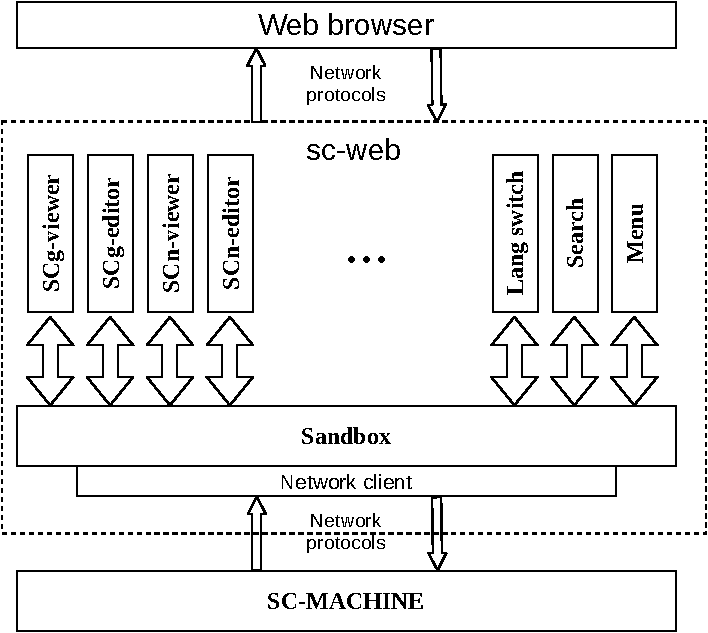
\includegraphics{figures/sd_interpreters/sc-web-new-arch.pdf}}}
\scnaddlevel{1}
	\scnexplanation{На данной иллюстрации показан планируемый вариант архитектуры \textit{Реализация интерпретатора sc-моделей пользовательских интерфейсов}, важным принципом которой является простота и однотипность подключения любых компонентов пользовательского интерфейса (редакторов, визуализаторов, переключателей, команд меню и т.д.). Для этого реализуется программная прослойка Sandbox, в рамках которой реализуются низкоуровневые операции взаимодействия с серверной частью и которая обеспечивает более удобный программный интерфейс для разработчиков компонентов.}
\scnaddlevel{-1}
\scnrelfromset{недостатки текущей реализации}{\scnfileitem{Отсутствие единого унифицированного механизма клиент-серверного взаимодействия. Часть компонентов (визуализатор sc-текстов в SCn-коде, команды меню и др.) работают по протоколу HTTP, часть по протоколу SCTP с использованием технологии WebSocket, это приводит к значительным трудностям при развитии платформы.};
\scnfileitem{Протокол HTTP предполагает четкое разделение активного клиента и пассивного сервера, который отвечает на запросы клиентов. Таким образом, сервер (в данном случае -- sc-память) практически не имеет возможности по своей инициативе отправить сообщение клиенту, что повышает безопасность системы, но значительно снижает ее интерактивность. Кроме того, такой вариант реализации затрудняет реализацию принятого в Технологии OSTIS многоагентного подхода, в частности, затрудняет реализацию sc-агентов на стороне клиента. Указанные проблемы могут быть решены путем постоянного мониторинга определенных событий со стороны клиента, однако такой вариант неэффективен.
Кроме того, часть интерфейса фактически работает напрямую с sc-памятью с использованием технологии WebSocket, а часть -- через прослойку на базе библиотеки tornado для языка программирования Python, что приводит к дополнительным зависимостям от сторонних библиотек.};
\scnfileitem{Часть компонентов (например, поле поиска по идентификатору) реализована сторонними средствами и практически никак не связана с sc-памятью. Это затрудняет развитие платформы.};
\scnfileitem{Текущая \textit{Реализация интерпретатора sc-моделей пользовательских интерфейсов} ориентирована только на ведение диалога с пользователем (в стиле вопрос пользователя -- ответ системы). Не поддерживаются такие очевидно необходимые ситуации, как выполнение команды, не предполагающей ответа\char59~возникновение ошибки или отсутствие ответа\char59~необходимость задания вопроса системой пользователю и т.д.};
\scnfileitem{Ограничена возможность взаимодействия пользователя с системой без использования специальных элементов управления. Например, можно задать вопрос системе, нарисовав его в SCg-коде, но ответ пользователь не увидит, хотя в памяти он будет сформирован соответствующим агентом.;
Большая часть технологий, использованных при реализации платформы, к настоящему моменту устарела, что затрудняет развитие платформы.};
\scnfileitem{Идея платформенной независимости пользовательского интерфейса (построения sc-модели пользовательского интерфейса) реализована не в полной мере. Полностью описать sc-модель пользовательского интерфейса (включая точное размещение, размеры, дизайн компонентов, их поведение и др.) в настоящее время скорее всего окажется затруднительно из-за ограничений производительности, однако вполне возможно реализовать возможность задания вопросов ко всем компонентам интерфейса, изменить их расположение и т.д., однако эти возможности нельзя реализовать в текущей версии реализации платформы.};
\scnfileitem{Интерфейсная часть работает медленно из-за недостатков  протокола SCTP и некоторых недостатков реализации серверной части на языке Python.};
\scnfileitem{Не реализован механизм наследования при добавлении новых внешних языков. Например, добавление нового языка даже очень близкого к SCg-коду требует физического копирования кода компонента и внесение соответствующих изменений, при этом получаются два никак не связанных между собой компонента, которые начинают развиваться независимо друг от друга.};
\scnfileitem{Слабый уровень задокументированности текущей \textit{Реализации интерпретатора sc-моделей пользовательских интерфейсов}.}}
\scnrelfromset{требования к будущей реализации}{\scnfileitem{Унифицировать принципы взаимодействия всех компонентов интерфейса с \textit{Программной моделью sc-памяти}, независимо от того, к какому типу относится компонент. Например, список команд меню должен формироваться через тот же механизм, что и ответ на запрос пользователя, и команда редактирования, сформированная пользователем, и команда добавления нового фрагмента в базу знаний и т.д.};
\scnfileitem{Унифицировать принципы взаимодействия пользователей с системой независимо от способа взаимодействия и внешнего языка. Например, должна быть возможность задания вопросов и выполнения других команд прямо через SCg/SCn интерфейс. При этом необходимо учитывать принципы редактирования базы знаний, чтобы пользователя не мог под видом задания вопроса внести новую информацию в согласованную часть базы знаний.};
\scnfileitem{Унифицировать принципы обработки событий, происходящих при взаимодействии пользователя с компонентами интерфейса -- поведение кнопок и других интерактивных компонентов должно задаваться не статически сторонними средствами, а реализовываться в виде агента, который, тем не менее, может быть реализован произвольным образом (не обязательно на платформенно-независимом уровне). Любое действие, совершаемое пользователем, на логическом уровне должно трактоваться и обрабатываться как инициирование агента.};
\scnfileitem{Обеспечить возможность выполнять команды (в частности, задавать вопросы) с произвольным количеством аргументов, в том числе -- без аргументов.};
\scnfileitem{Обеспечить возможность отображения ответа на вопрос по частям, если ответ очень большой и для отображения требуется много времени.};
\scnfileitem{Каждый отображаемый компонент интерфейса должен трактоваться как изображение некоторого sc-узла, описанного в базе знаний. Таким образом, пользователь должен иметь возможность задания произвольных вопросов к любым компонентам интерфейса.};
\scnfileitem{Максимально упростить и задокументировать механизм добавления новых компонентов.};
\scnfileitem{Обеспечить возможность добавления новых компонентов на основе имеющихся без создания независимых копий. Например, должна быть возможность создать компонент для языка, расширяющего язык SCg новыми примитивами, переопределять принципы размещения sc-текстов и т.д.};
\scnfileitem{Свести к минимуму зависимость от сторонних библиотек.};
\scnfileitem{Свести к минимуму использование протокола HTTP (начальная загрузка общей структуры интерфейса), обеспечить возможность равноправного двустороннего взаимодействия серверной и клиентской части.};
\scnfileitem{Полностью отказаться от протокола SCTP, перейти на протокол на базе JSON, задокументировать его.}}
\scnaddlevel{1}
	\scnnote{Очевидно, что реализация большинства из приведенных требований связана не только с собственно вариантом реализации платформы, но и требует развития теории логико-семантических моделей пользовательских интерфейсов и уточнения в рамках нее общих принципов организации пользовательских интерфейсов ostis-систем. Однако, принципиальная возможность реализации таких моделей должна быть учтена в рамках реализации платформы.}
\scnaddlevel{-1}
\scnrelfromlist{компонент программной системы}{Панель меню команд пользовательского интерфейса\\
	\scnaddlevel{1}
		\scnexplanation{\textit{Панель меню команд пользовательского интерфейса} содержит изображения классов команд (как атомарных, так и неатомарных), имеющихся на данный момент в базе знаний и входящих в декомпозицию \textit{Главного меню пользовательского интерфейса} (имеется в виду полная декомпозиция, которая в общем случае может включать несколько уровней неатомарных классов команд).\\
		Взаимодействие с изображением неатомарного класса команд инициирует команду изображения классов команд, входящих в декомпозицию данного неатомарного класса команд.\\
		Взаимодействие с изображением атомарного класса команд инициирует генерацию команды данного класса с ранее выбранными аргументами на основе соответствующей \textit{обобщенной формулировки класса команд} (шаблона класса команд).}
	\scnaddlevel{-1}
	;Компонент переключения языка идентификации отображаемых sc-элементов\\
	\scnaddlevel{1}
		\scnexplanation{\textit{Компонент переключения языка идентификации отображаемых sc-элементов} является изображением множества имеющихся в системе естественных языков. Взаимодействие пользователя с данным компонентом переключает пользовательский интерфейс в режим общения с конкретным пользователем с использованием \textit{основных sc-идентификаторов}, принадлежащих данному \textit{естественному языку}. Это значит, что при изображении sc-идентификаторов sc-элементов на каком-либо языке, например, SCg-коде или SCn-коде будут использоваться \textit{основные sc-идентификаторы}, принадлежащие данному \textit{естественному языку}. Это касается как sc-элементов, отображаемых в рамках \textit{Панели визуализации и редактирования знаний}, так и любых других sc-элементов, например, классов команд и даже самих \textit{естественных языков}, изображаемых в рамках самого \textit{Компонента переключения языка идентификации отображаемых sc-элементов}.}
	\scnaddlevel{-1}	
	;Компонент переключения внешнего языка визуализации знаний\\
	\scnaddlevel{1}
		\scnexplanation{\textit{Компонент переключения внешнего языка визуализации знаний} служит для переключения языка визуализации знаний в текущем окне, отображаемом на \textit{Панели визуализации и редактирования знаний}. В текущей реализации в качестве таких языков по умолчанию поддерживаются SCg-код и SCn-код, а также любые другие языки, входящие во множество \textit{внешних языков визуализации SC-кода}.}
	\scnaddlevel{-1}
	;Поле поиска sc-элементов по идентификатору\\
	\scnaddlevel{1}
		\scnexplanation{\textit{Поле поиска sc-элементов по идентификатору} позволяет осуществлять поиск sc-идентификаторов, содержащих подстроку, введенную в данное поле (с учетом регистра). В результате поиска отображается список sc-идентификаторов, содержащих указанную подстроку, при взаимодействии с которыми осуществляется автоматическое задание вопроса ``Что это такое?'', аргументом которого является либо для сам sc-элемент, имеющий данный sc-идентификатор (в случае, если указанный sc-идентификатор является основным или системным, и, таким образом, указанный sc-элемент может быть определен однозначно), либо для самого внутреннего файла ostis-системы, являющегося sc-идентификатором (в случае, если данный sc-идентификатор является неосновным).}
	\scnaddlevel{-1}
	;Панель отображения диалога пользователя с ostis-системой\\
	\scnaddlevel{1}
		\scnexplanation{\textit{Панель отображения диалога пользователя с ostis-системой} отображает упорядоченный по времени список sc-элементов, являющихся знаками действий, которые инициировал пользователь в рамках диалога с ostis-системой путем взаимодействия с изображениями соответствующих классов команд (то есть, если действие было инициировано другим способом, например, путем его явного инициирования через создание дуги принадлежности множеству \textit{инициированных действий} в sc.g-редакторе, то на данной панели оно отображено не будет). При взаимодействии пользователя с любым из изображенных знаков действий на \textit{Панели визуализации и редактирования знаний} отображается окно, содержащее результат выполнения данного \textit{действия} на том языке визуализации, на котором он был отображен, когда пользователь просматривал его в последний (предыдущий) раз. Таким образом, в текущей реализации данная панель может работать только в том случае, если инициированное пользователем действие предполагает явно представленный в памяти результат данного действия. В свою очередь, из этого следует, что в настоящее время данная панель, как и в целом \textit{Реализация интерпретатора sc-моделей пользовательских интерфейсов}, позволяет работать с системой только в режиме диалога ''вопрос-ответ''.}
	\scnaddlevel{-1}
	;Панель визуализации и редактирования знаний\\
	\scnaddlevel{1}
		\scnexplanation{\textit{Панель визуализации и редактирования знаний} отображает окна, содержащие sc-текст, представленный на некотором языке из множества \textit{внешних языков визуализации SC-кода} и, как правило, являющийся результатом некоторого действия, инициированного пользователем. Если соответствующий визуализатор поддерживает возможность редактирования текстов соответствующего естественного языка, то он одновременно является также и редактором.}
		\scnrelfromlist{компонент программной системы}{Визуализатор sc.n-текстов;Визуализатор и редактор sc.g-текстов}
		\scnnote{При необходимости пользовательский интерфейс каждой конкретной ostis-системы может быть дополнен визуализаторами и редакторами различных внешних языков, которые в текущей версии \textit{Реализации интерпретатора sc-моделей пользовательских интерфейсов} будут также располагаться на \textit{Панели визуализации и редактирования знаний}.}
	\scnaddlevel{-1}}

\scnheader{Реализация scp-интерпретатора}
\scnrelto{программная реализация}{Абстрактная scp-машина}
\scnnote{Важнейшей особенностью Языка SCP является тот факт, что его программы записываются таким же образом, что и обрабатываемые ими знания, то есть в SC-коде. Это, с одной стороны, дает возможность сделать ostis-системы платформенно-независимыми (четко разделить \textit{sc-модель компьютерной системы} и платформу интерпретации таких моделей), а с другой стороны требует наличия в рамках платформы \textit{Реализации scp-интерпретатора}, то есть интерпретатора программ Языка SCP.}
\scnrelfromlist{используемый язык программирования}{C++}
\scnrelfromlist{компонент программной системы}{Реализация Абстрактного sc-агента создания scp-процессов;Реализация Абстрактного sc-агента интерпретации scp-операторов\\
	\scnaddlevel{1}
	\scnrelfromlist{компонент программной системы}{Реализация Абстрактного sc-агента интерпретации scp-операторов генерации конструкций;Реализация Абстрактного sc-агента интерпретации scp-операторов ассоциативного поиска конструкций;Реализация Абстрактного sc-агента интерпретации scp-операторов удаления конструкций;Реализация Абстрактного sc-агента интерпретации scp-операторов проверки условий;Реализация Абстрактного sc-агента интерпретации scp-операторов управления значениями операндов;Реализация Абстрактного sc-агента интерпретации scp-операторов управления scp-процессами;Реализация Абстрактного sc-агента интерпретации scp-операторов управления событиями;Реализация Абстрактного sc-агента интерпретации scp-операторов обработки содержимых числовых файлов;Реализация Абстрактного sc-агента интерпретации scp-операторов обработки содержимых строковых файлов}
	\scnaddlevel{-1}
	;Реализация Абстрактного sc-агента синхронизации процесса интерпретации scp-программ;Реализация Абстрактного sc-агента уничтожения scp-процессов;Реализация Абстрактного sc-агента синхронизации событий в sc-памяти и ее реализации}
\scnnote{Текущая \textit{Реализация scp-интерпретатора} не включает в себя специализированных средств для работы с блокировками, поскольку механизм блокировок элементов sc-памяти реализован на более низком уровне в рамках \textit{Реализация sc-хранилища и механизма доступа к нему}}

\scnendstruct \scnendcurrentsectioncomment

\end{SCn}

\scsubsubsection{\textbf{Предметная область и онтология семантических ассоциативных компьютеров для ostis-систем}}
\label{sd_sem_comp}
\begin{SCn}

\scnsectionheader{\currentname}
\scnstartsubstruct

\scnheader{Предметная область и онтология семантических ассоциативных компьютеров для ostis-систем}
\scnsdmainclasssingle{***}
\scnsdclass{***}
\scnsdrelation{***}

\scnheader{семантический ассоциативный компьютер}
\scnidtf{аппаратно реализованный интерпретатор семантических моделей (sc-моделей) компьютерных систем}
\scnidtf{семантический ассоциативный компьютер, управляемый знаниями}
\scnidtf{компьютер с нелинейной структурно перестраиваемой (графодинамической) ассоциативной памятью, переработка информации в которой сводится не к изменению состояния элементов памяти, а к изменению конфигурации связей между ними}
\scnidtf{sc-компьютер}
\scnidtf{scp-компьютер}
\scnidtf{компьютер, управляемый знаниями, представленными в SC-коде}
\scnidtf{компьютер, ориентированный на обработку текстов SC-кода}

\scnrelfromlist{принцип}{
\scnfileitem{нелинейная память — каждый элементарный фрагмент хранимого в памяти текста может быть инцидентен неограниченному числу других элементарных фрагментов этого текста};
\scnfileitem{структурно перестраиваемая (реконфигурируемая) память — процесс отработки хранимой в памяти информации сводится не только к изменению состояния элементов, но и к реконфигурации связей между ними};
\scnfileitem{в качестве внутреннего способа кодирования знаний, хранимых в памяти семантического ассоциативного компьютера, используется универсальный (!) способ нелинейного (графоподобного) смыслового представления знаний, названный нами SC-кодом (семантическим, смысловым компьютерным кодом)};
\scnfileitem{обработка информации осуществляется коллективом агентов, работающих над общей памятью. Каждый из них реагирует на соответствующую ему ситуацию или событие в памяти (компьютер, управляемый хранимыми знаниями)};
\scnfileitem{есть программно реализуемые агенты, поведение которых описывается хранимыми в памяти агентно-ориентированными программами, которые интерпретируются соответствующими коллективами агентов;
есть базовые агенты, которые не могут быть реализованы программно (в частности, это агенты интерпретации агентных программ, базовые рецепторные агенты-датчики, базовые эффекторные агенты)};
\scnfileitem{все агенты работают над общей памятью одновременно. Более того, если для какого-либо агента в некоторый момент времени в различных частях памяти возникает сразу несколько условий его применения, разные акты указанного агента в разных частях памяти могут выполняться одновременно (акт агента — это неделимый, целостный процесс деятельности агента)};
\scnfileitem{для того, чтобы акты агентов, параллельно выполняемые в общей памяти не "мешали"{} друг другу, для каждого акта в памяти фиксируется и постоянно актуализируется его текущее состояние. То есть каждый акт сообщает всем остальным о своих намерениях и пожеланиях, которым остальные агенты не должны препятствовать (например, это различного рода блокировки используемых элементов семантической памяти)};
\scnfileitem{кроме того, агенты (точнее, выполняемые ими акты) должны соблюдать "этику"{}, стараясь не в ущерб себе создавать максимально благоприятные условия для других агентов (актов), например, не жадничать, быстрее возвращать, не захватывать (не блокировать) лишние элементы памяти, как можно скорее освобождать (деблокировать) заблокированные элементы памяти};
\scnfileitem{процессор и память семантического ассоциативного компьютера глубоко интегрированы и составляют единую процессоро-память. Процессор семантического ассоциативного компьютера равномерно "распределен"{} по его памяти так, что процессорные элементы одновременно являются и элементами памяти компьютера. Обработка информации в семантическом ассоциативном компьютере сводится к реконфигурации каналов связи между процессорными элементами,  следовательно память такого компьютера есть не что иное, как \uline{коммутатор} (!) указанных каналов связи. Таким образом, текущее состояние конфигурации этих каналов связи и есть текущее состояние обрабатываемой информации}}

\scntext{основная цель}{Повышение производительности систем, основанных на знаниях, представленных в виде семантических сетей}
\scnrelfromlist{решаемая задача}{
	разработка архитектуры интегрированного процессора (процессоро-памяти) семейства SCC (semantic code computer) для высокопроизводительной переработки знаний
	;аппаратная реализация интегрированного процессора и базового программного обеспечения SCC}
\scntext{актуальность}{Использование систем, основанных на знаниях, значительно повышает качество всех процессов, которые используют информацию}
	\scnaddlevel{1}
	\scnnote{Традиционная архитектура не позволяет эффективно использовать эти системы в реальном масштабе времени.
	
	Решение проблемы функционирования вычислительных систем обработки знаний в реальном масштабе времени трудно достижимо без использования принципов параллельной обработки и ассоциативного доступа к структурам данных. Разработка подобных систем чрезвычайно трудоемка, поэтому для обеспечения ее экономической целесообразности жизненный цикл функционирования подобных систем должен быть достаточно продолжительным (от десятка лет и более). Сменяемость аппаратных и программных средств вычислительной техники в настоящее время достигает от нескольких лет до нескольких месяцев. Это обусловливает необходимость наличия у \textit{интеллектуальных систем} таких качеств, как:
	\begin{scnitemize}
	\item открытость (в плане модифицируемости и добавления новых методов представления и переработки знаний);
	\item интегрируемость (в смысле возможности функционирования в составе комплексов различных вычислительных и исполнительных средств).
	\end{scnitemize}	   
	Анализ современных систем обработки знаний показывает, что ни одна из архитектур, на базе которых они реализованы, не обладает в совокупности всеми указанными выше свойствами.}
		\scnaddlevel{1}
		\scnnote{Особенности логической организации вычислительных систем, которые существенно затрудняют создание машин переработки знаний на основе традиционных ЭВМ:
		\begin{scnitemize}
		\item последовательная обработка, ограничивающая эффективность ЭВМ физическими возможностями элементной базы;
		\item низкий уровень доступа к памяти, т.е. сложность и громоздкость выполнения процедуры ассоциативного поиска нужного фрагмента знаний. 
		\item линейная организация памяти и чрезвычайно простой вид конструктивных объектов, непосредственно хранимых в памяти. Это приводит к тому, что в интеллектуальных системах, построенных на базе современных ЭВМ, манипулирование знаниями осуществляется с большим трудом. Во-первых, приходится оперировать не самими структурами, а их громоздкими линейными представлениями (списками, матрицами смежности, матрицами инцидентности); во-вторых, линеаризация сложных структур разрушает локальность их преобразований;
		\item представление информации в памяти современных ЭВМ имеет уровень весьма далекий от семантического, что делает переработку знаний довольно громоздкой, требующей учета большого количества деталей, касающейся не смысла перерабатываемой информации, а способа ее представления в памяти;
		\item в современных ЭВМ имеет место весьма низкий уровень аппаратно реализуемых операций над нечисловыми данными и полностью отсутствует аппаратная поддержка логических операций над фрагментами знаний, имеющих сложную структуру, что делает манипулирование такими фрагментами весьма сложным.

		\end{scnitemize}
	
	Основным проявлением перечисленных недостатков традиционных ЭВМ является гипертрофированное развитие программного обеспечения, сложность его создания и невысокая надежность.
	
	Трудности, связанные с использованием универсальных многопроцессорных ЭВМ, послужили толчком к развитию теоретических исследований в области параллельного программирования.}
		\scnaddlevel{-1}
	\scnaddlevel{-1}
\scnrelfrom{предлагаемый подход}{\scnkeyword{SC-код}}
	\scnaddlevel{1}
	\scnidtf{Предлагаемое в рамках \textit{Технологии OSTIS} уточнение понятия \textit{семантической сети}}
	\scnidtf{Semantic Computer Code}
	\scnnote{\textit{Semantic Code} обладает фиксированными синтаксисом и денотационной семантикой, но нефиксированной операционой семантикой. Следовательно, позволил на его основе создать семейство языков представления знаний различного вида.}
	\scnaddlevel{-1}

	
\scnheader{информационно-логические задачи}
\scnidtf{информационно-логические и комбинаторные задачи по переработке сложноструктурированных баз данных}
\scnidtf{класс задач, предполагающих переработку нечисловой сложноструктурированной информации и допускающих при этом отсутствие точного алгоритма их решения}
\scnnote{Понятие информационно-логических задач фактически совпадает по смыслу с широко используемым в последнее время понятием задач искусственного интеллекта, что позволяет использовать оба эти термина.}

\scnnote{Разработка средств решения задач того или иного класса в настоящее время обычно осуществлявшая путем создания языка программирования высокого уровня, ориентированного на этот класс задач, и путем реализации такого языка на современных ЭВМ, т.е. путем создания транслятора. Поскольку логика решения задач искусственного интеллекта плохо согласуется с современными языками программирования, более целесообразной является разработка принципиально новых языков, отражающих на уровне их элементарных операций основные логические механизмы решения задач рассматриваемого класса. Такие языки программирования обычно называют языками сверх-высокого уровня или непроцедурными языками. Реализация языков сверх-высокого уровня на современных ЭВМ представляется весьма сложной в силу большого разрыва между языками этого класса и внутренними языками современных ЭВМ, для преодоления которого создание эффективного транслятора оказывается практически невозможным.}
\scnaddlevel{1}
\scnexplanation{Таким образом, состояние проблемы автоматизации решения задач искусственного интеллекта (информационно-логических задач) в настоящее время можно охарактеризовать тем, что эта проблема входит в противоречие c принципами логической организации современных ЭВМ и, в первую очередь, с используемыми в современных ЭВМ внутренними языками. 

Причины плохой приспособленности современных ЭВМ к решению информационно-логических задач:
	\begin{scnitemize}
		\item в современных ЭВМ при работе со сложноструктурированными базами данных время, затрачиваемое на информационный поиск, на 2—3 порядка превышает время, затрачиваемое на собственно переработки;
		\item в современных ЭВМ имеет место весьма низкий уровень аппаратурно реализуемых операций над нечисловыми данными;
		\item представление информации в памяти современных ЭВМ имеет уровень весьма далекий от семантического, что делает переработку информации довольно громоздкой, требующей учета большого количества деталей, касающихся не смысла перерабатываемой информации, a способа ее представления в памяти;
		\item в современных ЭВМ громоздка реализуются даже простейшие процедуры логического вывода.
	\end{scnitemize}

Перечисленные причины, по существу, не устраняются также и в развиваемых в настоящее время подходах к построению нетрадиционных высокопроизводительных ЭВМ, ибо, в основном, все эти подходы (даже если они достаточно далеко отходят от предложенных фон Нейманом принципов организации вычислительных машин) неявно сохраняют точку зрения на ЭВМ как на большой арифмометр и тем самым сохраняют ее ориентацию на задачи числового характера. Очевидно, что эффективность этих машин будет прежде всего определяться степенью близости их внутреннего языка к языкам непроцецурного типа (к языкам сверх-высокого уровня). Учитывая указанное назначение таких машин, их естественно назвать не вычислительными машинами, a математическими машинами или даже «мыслительными» машинами.}
\scnaddlevel{-1}

\scnrelfrom{предлагаемый подход}{подход к построению машин, ориентированных на решение информационно-логических задач}

\scnheader{подход к построению машин, ориентированных на решение информационно-логических задач}
\scnidtf{стремление так организовать процесс переработки информации, чтобы он был наиболее близок к семантическому (содержательному) уровню}
\scnrelfromlist{требование}{
	\scnfileitem{разработка семантического способа представления перерабатываемой информации в памяти машины};
	\scnfileitem{разработка такого внутреннего языка, запись программ на котором была бы максимально близка к тому, что называют записью алгоритма на содержательном уровне};
	\scnfileitem{разработка и исследование способов семантического представления информации различного вида};
	\scnfileitem{разработка и исследование принципов организации развитой ассоциативной памяти для непосредственного хранения семантического представления информации};
	\scnfileitem{разработка и исследование языка программирования высокого уровня, который (I) ориентирован на решение информационно-логических задач; (2) обеспечивает непосредственную реализацию простых процедур логического вывода. (3) согласован c выбранным способом семантического представления перерабатываемой информации, (4) приспособлен к использованию в качестве внутреннего языкё параллельной однородной структуры, имеющей распределенную ассоциативную память для хранения сложноструктурированных данных};
	\scnfileitem{разработка и исследование принципов построения и‚ принципов параллельного взаимодействия функциональных средств, обеспечивающих непосредственную переработку семантического представления информации в распределенной ассоциативной памяти и реализующих управление потоком словноструктурированных данных};
	\scnfileitem{экспериментальная проверка полученных результатов}
}
\scnnote{Исследования по системам искусственного интеллекта убедительно показали, что способ представления знаний в их памяти, точнее степень его близости к семантическому, является фактором, во многом определяющим эффективность таких систем.}
\scnrelfromlist{принципы построения}{
	\scnfileitem{такие машины целесообразно строить как машины, манипулирующие графовыми структурами непосредственно на физическом уровне}
	\scnaddlevel{1}
	\scnexplanation{Предполагается создание структурно-перестраиваемой («графовой») памяти. Такая память состоит из ячеек, однозначно соответствующих вершинам хранимого в памяти графа, но, в отличие от обычной памяти, эти ячейки связываются не фиксированными условными связями, задающими фиксированную последовательность (порядок) ячеек в памяти, a реально (физически) проводимыми связями произвольной конфигурации. Эти связи соответствуют дугам, ребрам, гиперребрам записанного в памяти графа. Очевидно, что в ходе переработки информации в структурно-перестраиваемой памяти меняются на только и даже не столько состояния ячеек памяти, как это имеет место в обычной памяти, сколько конфигурация связей между этими ячейками. Т.е. в структурно-перестраиваемой памяти в ходе переработки информации не только перераспределяются метки на вершинах записанного в памяти графа, но и меняется структура самого этого графа.}
	\scnaddlevel{-1};
	\scnfileitem{в качестве внутреннего языка таких машин целесообразно использовать язык типа PROLOG.}
	\scnaddlevel{1}
	\scnexplanation{Разработка языка типа PROLOG, предназначенного к использованию в качестве внутреннего языка программирования для машин co структурно-перестраиваемой памятью‚ требует решения нетривиальной задачи согласования графового способа представления данных в структурно-перестраиваемой памяти и способа записи в этой же памяти самих программ, описывающих переработку этих данных. Переход на «графовый» способ кодирования программ и данных в структурно-перестраиваемой памяти обеспечивает компактность их представления и существенно упрощает аппаратурную реализацию операций над сложными структурами. Говоря об аппаратурной интерпретации языка типа PROLOG‚ необходимо подчеркнуть следующее. На уровне любого языка типа PROLOG, т.е. на уровне абстрактной PROLOG — машины‚ естественным образом реализуется эффективное распараллеливание процесса переработки сложных структур, организованное по принципу управления потоком запросов или управления потоком перерабатываемых сложноструктурированных данных. Управление потоком сложноструктурированных данных при этом основывается на использовании развитой формы ассоциативного доступа, a именно, доступа к произвольному фрагменту перерабатываемых данных (фрагменту, имеющему произвольный размер и произвольную структуру). Из вышесказанного следует, что создание машины, аппаратурно интерпретирующей язык типа PROLOG, есть не что иное, как создание параллельной машины, управляемой потоком сложноструктурированных данных и имеющей развитую ассоциативную память.}
	\scnaddlevel{-1};
	\scnfileitem{принцип организации переработки информации непосредственно в памяти}
	\scnaddlevel{1}
	\scnexplanation{Этот принцип обеспечивает значительное ускорение переработки информации благодаря исключению этапов передачи информации из памяти в процессор и обратно, но оплачивается ценой большой избыточности функциональных (процессорных; средств, равномерно распределяемых по памяти. При распределении функциональных средств по структурно-перестраиваемой памяти каждая ячейка дополняется функциональным (процессорным) элементом, a перестраиваемые связи между ячейками становятся коммутируемыми каналами связи между функциональными элементами. Каждый функциональный элемент при этом имеет свою специальную внутреннюю регистровую память, отражающую важные для данного функционального элемента аспекты текущего состояния процесса выполнения элементарных операций внутреннего языка.}
	\scnaddlevel{-1}
}
\scntext{методы исследования}{сочетание теории множеств, теории алгебраических систем, теории графов, математической логики, теории вычислений, методов машинного моделирования}

\scnrelfromlist{основные положения}{
	\scnfileitem{теорию наиболее общего вида структур данных (квази-графов), используемых в задачах искусственного интеллекта и являющихся обобщением классических алгебраических моделей};
	\scnfileitem{ориентированный на аппаратурную интерпретацию способ кодирования сложноструктурированных данных (квази-графв) в виде однородных семантических сетей специального вида};
	\scnfileitem{новый логический язык, являющийся модификацией классического и обеспечивающий описание квази-графов};
	\scnfileitem{графовые варианты логического языка описания квази-графов и, в частности, ориентированный на аппаратурную интерпретацию способ кодирования логических формул в виде однородных семантических сетей};
	\scnfileitem{непроцецурный язык программирования типа PROLOG, отличающийся удобством работы со сложными структурами данных (квази-графами) и развитостью средств управления вычислительным процессом};
	\scnfileitem{предлагаемый в качестве внутреннего аппаратурно интерпретируемого языка программирования способ записи непроцедурных программ в виде однородных семантических сетей};
	\scnfileitem{архитектуру и принципы организации однородной ассоциативной параллельной структуры, ориентированной на переработку семантических сетей и обеспечивающей аппаратурную интерпретацию непроцецурного языка программирования типа PROLOG}
}
\scnnote{Впервые исследованы пути построения параллельных машин, управляемых потоком сложноструктурированных данных. В качестве памяти таких машин впервые предложена структурно-перестраиваемая запоминающая среда, обеспечивающая непосредственное хранение графовых структур и манипулирование ими, a также обеспечивающая ассоциативный доступ к произвольным фрагментам перерабатываемых графовых структур (фрагментам, имеющим произвольный вид и произвольный размер). Впервые проведено исследование путей и принципов аппаратурной интерпретации непроцецурных языков программирования типа PROLOG. B качестве интерпретируемого (внутреннего) языка впервые предложен и исследован язык программирования графового типа, являющийся способом записи программ в виде однородных семантических сетей.}
\scnnote{Результаты работы могут быть использованы при выборе внутреннего языка, способа организации памяти и архитектуры вычислительных машин 5-го поколения, ориентированных на решение задач искусственного интеллекта и приспособленных к переработке сложноструктурированных данных. Результаты работы могут служить основой для формулирования заданий на опытно-конструкторские разработки по созданию вычислительных машин указанного класса. Использование результатов работы позволит:
	\begin{scnitemize}
		\item существенно расширить класс аппаратурно интерпретируемых (непосредственно перарабатываемых) структур данных;
		\item обеспечить высокую скорость переработки сложноструктурированных данных, благодаря (1) «укрупнению» аппаратурно реализуемых операций преобразования структур данных, (2) глубокому распараллеливанию процесса переработки сложных структур как на программном, так и на микропрограммном уровне, (3) организации переработки информации непосредственно в памяти;
		\item представление информации в памяти современных ЭВМ имеет уровень весьма далекий от семантического, что делает переработку информации довольно громоздкой, требующей учета большого количества деталей, касающихся не смысла перерабатываемой информации, a способа ее представления в памяти;
		\item существенно расширить логические возможности вычислительных машин благодаря использованию логического языка в качестве основы внутреннего языка программирования;
		\item обеспечить достаточно высокую технологичность вычислительных машин рассматриваемого класса благодаря их организации как однородных структур.
	\end{scnitemize}
}
\bigskip

\scnendstruct \scnendcurrentsectioncomment

\end{SCn}

\scsubsection{\textbf{Предметная область и онтология Библиотеки многократно используемых компонентов ostis-систем}}
\begin{SCn}

\scnsectionheader{\currentname}
\scnrelfromlist{подраздел}{Предметная область и онтология многократно используемых компонентов баз знаний ostis-систем;Предметная область и онтология многократно используемых внутренних агентов ostis-систем;Предметная область и онтология многократно используемых интерпретируемых ostis-системами методов;Предметная область и онтология многократно используемых компонентов интерфейсов ostis-систем;Библиотека многократно используемых встраиваемых ostis-систем}

\scnstartsubstruct

\scnheader{Предметная область многократно используемых компонентов ostis-систем}
\scnsdmainclasssingle{...}
\scnsdclass{}
\scnsdrelation{}

\scnheader{Библиотека многократно используемых компонентов OSTIS}
\scnidtf{Библиотека OSTIS}
\scnidtf{многократно используемый компонент OSTIS}
\scnidtf{многократно используемый компонент интеллектуальных систем, построенных по Технологии OSTIS}
\scnexplanation{Под \textbf{\textit{многократно используемым компонентом OSTIS}} понимается компонент некоторой ostis-системы, который может быть использован в рамках другой ostis-системы. Для этого необходимо выполнение как минимум двух условий:
\begin{scnitemize}
    \item есть техническая возможность встроить компонент в другую ostis-систему, либо путем физического копирования, переноса и встраивания его в проектируемую систему, либо использования компонента, размещенного в исходной системе наподобие сервиса, то есть без явного копирования и переноса компонента. Трудоемкость встраивания зависит, в том числе, от реализации компонента;
    \item использование компонента в каких-либо ostis-системах, кроме материнской, является целесообразным, то есть компонентом не может быть частное решение, ориентированное на узкий круг задач. Стоит, однако, отметить, что в общем случае практически каждое решение может быть использовано в каких-либо других системах, круг которых определяется степенью общности и предметной зависимостью такого решения.
\end{scnitemize}
С формальной точки зрения каждый \textbf{\textit{многократно используемый компонент OSTIS}} представляет собой \textit{структуру}, которая содержит все те (и только те) \textit{sc-элементы}, которые необходимы для функционирования компонента в \textit{дочерней ostis-системе} и, соответственно, должны быть в нее скопированы при включении компонента в одну из таких систем. Конкретный состав данной \textit{структуры} зависит от типа компонента и уточняется для каждого типа отдельно. По сути, данная \textit{структура} представляет собой эталон или образец, который копируется при включении соответствующего компонента в дочернюю систему.

Каждый \textbf{\textit{многократно используемый компонент OSTIS}} может быть атомарным, либо неатомарным, то есть состоять из более простых самодостаточных компонентов.

В зависимости от типа компонента в его составе, т.е. в составе соответствующей \textit{структуры}, могут дополнительно вводиться роли некоторых \textit{sc-элементов}, если это необходимо. Например, в случае \textit{многократно используемого sc-агента}, сам \textit{sc-узел}, обозначающий \textit{sc-агент}, будет являться \textit{ключевым sc-элементом'} в рамках компонента.

В каждый момент времени в текущем состоянии \textit{sc-памяти} каждый многократно используемый компонент может представлен полностью, т.е. в памяти явно присутствуют все \textit{sc-дуги принадлежности}, соединяющие соответствующую компоненту \textit{структуру} и все ее элементы, или представлен неявно, например, при помощи указания \textit{ключевых sc-элементов'} данного компонента или путем задания декомпозиции данного компонента на более частные.

Каждый \textbf{\textit{многократно используемый компонент OSTIS}} имеет формальную спецификацию, то есть некоторую \textit{семантическую окрестность}, характеризующую данный компонент. На основе формальной спецификации осуществляется поиск подходящего компонента в библиотеке, сравнение его с другими компонентами и т.д.

Данная спецификация включает, как минимум:
\begin{scnitemize}
    \item Информацию об авторстве компонента, то есть связь компонента со знаком автора (физического лица, коллектива и т.д.) при помощи отношения \textit{автор*};
    \item Информацию о типе компонента, посредством указания принадлежности компонента какому-либо классу многократно используемых компонентов;
    \item Описание назначения компонента, его особенностей;
    \item Историю изменений компонента по версиям;
    \item При необходимости сведения об открытости компонента и возможностях его использования в различных системах с точки зрения проприетарности;
    \item И др.
\end{scnitemize}
Не следует путать понятия \textbf{версии компонента} и \textbf{модификации компонента}. Версии отражают историю изменений компонента (как правило, какие-либо улучшения или устранения ошибок). Модификации представляют собой функционально эквивалентные, но разные варианты реализации одного и того же компонента, которые могут быть синтаксически эквивалентны (то есть быть реализованными при помощи одних и тех же языковых средств). В качестве примера синтаксически не эквивалентной модификации можно привести реализацию одного и того же \textit{sc-агента} на одном и том же языке но с отличиями в алгоритме, в качестве синтаксически эквивалентной модификации – платформенно-зависимую и платформенно-независимую реализацию одного и того же \textit{sc-агента}.

В общем случае система \textit{IMS} как материнская система взаимодействует со всеми своими \textit{дочерними ostis-системами} (с системами, построенными по \textit{Технологии OSTIS}), обеспечивая в дочерних системах автоматическое обновление версий \textit{многократно используемых компонентов OSTIS}. Любая дочерняя система, построенная по \textit{Технологии OSTIS}, в том числе, выполняет роль посредника между разработчиком такой системы и системой \textit{IMS}. Разработчик имеет возможность выбрать интересующий его компонент или набор компонентов в одной из библиотек, и включить их в разрабатываемую дочернюю систему. Таким образом, можно говорить о том, что \textbf{разработчик} систем, построенных по \textit{Технологии OSTIS}, является \textbf{конечным пользователем} системы \textit{IMS}. При обеспечении такого механизма взаимодействия между системами, построенными на основе \textit{Технологии OSTIS}, указанные системы формируют Глобальную базу знаний, в пределах которой различные системы могут координироваться и решать более глобальные задачи, нежели это может делать одна отдельно взятая система. В случае намеренной изоляции какой-либо из систем из такого коллектива, в частности, потери связи с системой \textit{IMS}, она теряет возможность получать своевременные обновления используемых компонентов, а также использовать знания, накопленные в других системах для решения стоящих перед ней задач. Речь в данном случае идет не только о физической изоляции рассматриваемой системы, которая может быть легко устранена, а о рассогласовании знаний данной системы и других систем, что не позволит безболезненно интегрировать компоненты из библиотек в такую систему. Таким образом, разработчик каждой системы обязан следить за тем, чтобы его система находилась в постоянном согласовании с глобальным смысловым пространством, что позволит пользователям в полной мере использовать все возможности коллектива систем.

В некоторых случаях может оказаться, что для использования одного \textbf{\textit{многократно используемого компонента OSTIS}} целесообразно или даже необходимо дополнительно использовать несколько других \textbf{\textit{многократно используемых компонентов OSTIS}}. Например, может оказаться целесообразным вместе с каким либо \textit{sc-агентом информационного поиска} использовать соответствующую команду интерфейса, которая представлена отдельным компонентом и позволит пользователю задавать вопрос для указанного \textit{sc-агента} через интерфейс системы. В таких случаях для связи компонентов используется отношение \textit{сопутствующий компонент*}. Наличие таких связей позволяет устранить возможные проблемы неполноты знаний и навыков в дочерней системе, из-за которых какие-либо из компонентов могут не выполнять свои функции. Связки отношения \textit{сопутствующий компонент*} связывают \textbf{\textit{многократно используемые компоненты OSTIS}}, которые целесообразно или необходимо использовать в дочерней системе вместе. При этом каждая связка направляется от зависящего компонента к зависимому. Каждая такая связка может дополнительно быть снабжена \textit{комментарием} или \textit{пояснением}, отражающим суть указываемой зависимости.

Включение компонента в \textit{дочернюю ostis-систему} в самом общем случае состоит из следующих этапов:
\begin{scnitemize}
    \item поиск подходящего компонента (или набора компонентов) во множестве библиотек, входящих в состав \textit{IMS}. Для облегчения задачи поиска могут быть реализованы специализированные поисковые агенты. В любом случае, поиск и выделение компонента будет осуществляться на основе спецификации компонента. Данный этап с точки зрения пользователя не зависит от типа компонента и особенностей его реализации. Конкретные действия на следующих  этапах сильно зависят от реализации и типа компонента и будут более детально описаны при рассмотрении подклассов \textbf{\textit{многократно используемых компонентов OSTIS}};
    \item выделение компонента (или набора компонентов) в рамках \textit{IMS} в виде, удобном для транспортировки в \textit{дочернюю ostis-систему} (при необходимости – создание физической копии компонента);
    \item транспортировка выделенного компонента в \textit{дочернюю sc-систему};
    \item интеграция компонента в \textit{дочернюю ostis-систему}. Если в системе уже использовалась более старая версия компонента, то необходимо произвести либо локальное обновление, либо полную замену устаревшей версии компонента. Дальнейший процесс интеграции зависит от типа компонента, например, в случае добавления нового \textit{sc-агента} он должен быть помечен как \textit{активный sc-агент} и т.п.
\end{scnitemize}

Для обеспечения возможности встраивания \textbf{\textit{многократно используемых компонентов OSTIS}} в дочернюю систему, каждая такая система обязана иметь в своем составе средства, обеспечивающие интеграцию новых компонентов в систему и, при необходимости, удаление устаревших версий этих компонентов (или автоматического локального обновления компонентов до более новой версии).}

\scnauthorcomment{разбиение согласовать со структурой разделов или убрать вообще}

\scnsubdividing{Семейство платформ интерпретации sc-моделей компьютерных систем
;Библиотека многократно используемых компонентов sc-моделей баз знаний;Библиотека шаблонов типовых компонентов sc-моделей компьютерных систем;Библиотека многократно используемых компонентов абстрактных sc-машин;Библиотека многократно используемых компонентов sc-моделей интерфейсов компьютерных систем;Библиотека типовых подсистем компьютерных систем, разрабатываемых по Технологии OSTIS}
\scnsubdividing{атомарный многократно используемый компонент OSTIS;неатомарный многократно используемый компонент OSTIS}
\scnsubdividing{платформенно-зависимый многократно используемый компонент OSTIS;платформенно-независимый многократно используемый компонент OSTIS}

\scnheader{шаблон типового компонента OSTIS}

\scnheader{атомарный многократно используемый компонент OSTIS}
\scnexplanation{Под \textbf{\textit{атомарным многократно используемым компонентом OSTIS}} подразумевается компонент, который в текущем состоянии библиотеки компонентов рассматривается как неделимый, то есть не содержит в своем составе других компонентов, представленных в какой-либо из библиотек компонентов в рамках \textit{IMS}. В общем случае атомарный компонент может перейти в разряд неатомарных в случае, если будет принято решение выделить какую-то из его частей в качестве отдельного компонента. Все вышесказанное, однако, не означает, что даже в случае его платформенной независимости, атомарный компонент всегда хранится в sc-памяти как сформированная sc-структура. Например, \textit{платформенно-независимая реализация sc-агента} всегда будет представлена набором \textit{scp-программ}, но будет \textbf{\textit{атомарным многократно используемым компонентом OSTIS}} в случае, если ни одна из этих программ не будет представлять интереса как самостоятельный компонент.}

\scnheader{неатомарный многократно используемый компонент OSTIS}
\scnexplanation{Под \textbf{\textit{неатомарным многократно используемым компонентом OSTIS}} подразумевается компонент, который в текущем состоянии библиотеки компонентов содержит в своем составе более простые компоненты, представленные в каких-либо библиотеках компонентов в рамках \textit{IMS}. В общем случае неатомарный компонент может перейти в разряд атомарных в случае, если будет принято решение по каким-либо причинам исключить все его части из рассмотрения в качестве отдельных компонентов.

Следует отметить, что неатомарный компонент необязательно должен складываться полностью из других компонентов, в его состав могут также входить и части, не являющиеся самостоятельными компонентами. Например, в состав реализованного на \textit{языке SCP sc-агента}, являющего \textbf{\textit{неатомарным многократно используемым компонентом}} могут входить как \textit{scp-программы}, которые могут являться \textit{многократно используемыми компонентами} (а могут и не являться), а также \textit{агентная scp-программа}, которая не имеет смысла как многократно используемый компонент.}

\scnheader{платформенно-зависимый многократно используемый компонент OSTIS}
\scnexplanation{Под \textbf{\textit{платформенно-зависимым многократно используемым компонентом OSTIS}} понимается компонент, частично или полностью реализованный при помощи каких-либо сторонних с точки зрения \textit{Технологии OSTIS} средств. Основной недостаток платформенно-зависимых компонентов состоит в том, что их интеграция в интеллектуальные системы может сопровождаться дополнительными трудностями, зависящими от конкретных средств реализации компонента. В качестве возможного преимущества \textbf{\textit{платформенно-зависимых многократно используемых компонентов OSTIS}} можно выделить их, как правило, более высокую производительность за счет реализации их на более приближенном к платформе уровне.

В общем случае \textbf{\textit{платформенно-зависимый многократно используемый компонент OSTIS}}  может поставляться как в виде набора исходных кодов, так и бинарном виде, например в виде скомпилированной библиотеки.

Процесс интеграции \textbf{\textit{платформенно-зависимого многократно используемого компонента OSTIS}} в дочернюю систему, разработанную по \textit{Технологии OSTIS}, сильно зависит от технологий реализации данного компонента и в каждом конкретном случае может состоять из различных этапов.

Для того чтобы \textbf{\textit{платформенно-зависимый многократно используемый компонент OSTIS}} мог быть успешно встроен в дочернюю систему, необходимо выполнение следующих условий:
\begin{scnitemize}
    \item в состав \textit{структуры}, соответствующей компоненту, должны входить знаки \textit{файлов}, обозначающих исходные тексты компонента или уже собранной его версии, то есть ссылки на внешние ресурсы или явно включенные в систему файлы компонента в виде указанных \textit{файлов};
    \item каждый \textbf{\textit{платформенно-зависимый многократно используемый компонент OSTIS}} должен иметь соответствующую подробную, корректную и понятную инструкцию по его установке и внедрению в дочернюю систему;
\end{scnitemize}
}

\scnheader{платформенно-независимый многократно используемый компонент OSTIS}
\scnexplanation{Под \textbf{\textit{платформенно-независимым многократно используемым компонентом OSTIS}} понимается компонент, который целиком и полностью представлен в \textit{SC-коде}. В случае \textit{неатомарного многократно используемого компонента} это означает, что все более простые компоненты, входящие в его состав также обязаны быть \textbf{\textit{платформенно-независимыми многократно используемыми компонентами OSTIS}}.

Процесс интеграции \textbf{\textit{платформенно-зависимого многократно используемого компонента OSTIS}} в дочернюю систему, разработанную по \textit{Технологии OSTIS}, существенно упрощается за счет использования общей унифицированной формальной основы представления и обработки знаний.

В случае \textbf{\textit{платформенно-независимого многократно используемого компонента OSTIS }} процесс интеграции конкретизируется до следующих этапов:
\begin{scnitemize}
    \item формирование \textit{структуры}, явно содержащей все \textit{sc-элементы}, входящие в состав компонента, а также все \textit{sc-элементы}, входящие в спецификацию компонента, необходимую для его функционирования в дочерней системе. В случае \textbf{\textit{неатомарного многократно используемого компонента OSTIS}} в указанную \textit{структуру} должны быть полностью включены и все более частные компоненты;
    \item транспортировка компонента в дочернюю систему. В худшем случае может быть осуществлена путем выгрузки всей \textit{структуры} компонента в какой-либо формат, например \textit{SCs-код}, с последующим переносом файла в дочернюю систему разработчиком вручную. В общем случае, дочерняя система по команде разработчика должна самостоятельно обращаться к родительской и осуществлять загрузку необходимых компонентов;
    \item интеграция нового компонента в \textit{дочернюю ostis-систему} либо обновление компонента с более старой версии. Если функция обновления не поддерживается, то интеграция может проводиться в два этапа – удаление старой версии компонента и добавление в систему более новой версии. В зависимости от типа компонента (\textit{многократно используемый компонент баз знаний} или \textit{многократно используемый компонент машин обработки знаний}) интеграция осуществляется по-разному.
\end{scnitemize}
}

\scnheader{Библиотека многократно используемых компонентов абстрактных sc-машин}
\scnidtf{многократно используемый компонент абстрактных sc-машин обработки знаний}
\scntext{примечание}{Если \textbf{\textit{многократно используемый компонент абстрактных sc-машин обработки знаний}} является \textit{платформенно-зависимым многократно используемым компонентом OSTIS}, то его интеграция производится в соответствии с инструкцией, как и для любого компонента такого рода. В противном случае, процесс интеграции можно конкретизировать в зависимости от подклассов данного типа компонентов.}
\scnsubdividing{Библиотека многократно используемых абстрактных sc-агентов;Библиотека многократно используемых программ обработки sc-текстов}

\scnheader{шаблон типового компонента sc-моделей компьютерных систем}
\scnidtf{образец типового компонента OSTIS}
\scnidtf{атомарная логическая формула, описывающая структуру аналогичных (чаще всего изоморфных) компонентов баз знаний ostis-систем}
\scnidtf{Библиотека шаблонов типовых компонентов sc-моделей компьютерных систем}
\scnexplanation{В процессе использования \textbf{\textit{шаблона типового компонента sc-моделей компьютерных систем}} при формировании баз знаний проектируемых \textit{ostis-систем} вместо \textit{sc-переменных}, входящих в состав компонента, подставляются их значения.}

\scnheader{сопутствующий компонент*}

\scnheader{декомпозиция компонента библиотеки*}
\scniselement{квазибинарное отношение}
\scniselement{отношение декомпозиции}

\scnendstruct

\end{SCn}
\scsubsubsection{Предметная область и онтология Библиотеки многократно используемых компонентов баз знаний ostis-систем}
\begin{SCn}

\scnsectionheader{\currentname}
\scnsuperset{Предметная область многократно используемых компонентов баз знаний ostis-систем}
\scnaddlevel{1}
\scnsdmainclasssingle{...}
\scnsdclass{}
\scnsdrelation{}
\scnaddlevel{-1}

\scnstartsubstruct

\scnheader{Библиотека многократно используемых компонентов sc-моделей баз знаний}
\scnidtf{многократно используемый компонент sc-моделей баз знаний}
\scnexplanation{Каждый \textbf{\textit{многократно используемый компонент sc-моделей баз знаний}} представляет собой \textit{структуру}, либо явно представленную в текущем состоянии \textit{sc-памяти}, либо не полностью сформированную \textit{структуру}, которая при необходимости может быть полностью сформирована путем объединения своих частей, указанных при помощи какого-либо \textit{отношения декомпозиции}, например \textit{разбиение*}, или отношения \textit{включение*}.

Интеграция \textbf{\textit{многократно используемого компонента sc-моделей баз знаний}} в дочернюю систему сводится к склеиванию ключевых узлов по идентификаторам и устранению возможных дублирований и противоречий, которые могли возникнуть в случае, если разработчик дочерней системы вручную вносил какие-либо изменения в ее базу знаний.

К основным типам компонентов баз знаний, хранящихся в библиотеке компонентов баз знаний, относятся:
\begin{scnitemize}
    \item онтологии различных предметных областей, которые могут быть самыми различными по содержанию, однако должны быть семантически совместимыми;
    \item базовые фрагменты теорий, соответствующие различным уровням знания пользователя, начиная от базового школьного до профессионального;
    \item различные \textit{семантические окрестности} различных объектов;
    \item спецификации формальных \textit{sc-языков}, соответствующих различным \textit{предметным областям}.
\end{scnitemize}

Для обеспечения семантической совместимости компонентов баз знаний, которые являются унифицированными семантическими моделями, необходимо
\begin{scnitemize}
    \item согласовать семантику всех используемых ключевых узлов;
    \item согласовать \textit{системные идентификаторы*} ключевых узлов, используемых в разных компонентах. После этого интеграция всех компонентов, входящих в состав библиотеки, и в любых комбинациях осуществляется автоматически, без вмешательства разработчика.
\end{scnitemize}
Для включения компонента в библиотеку необходимо его специфицировать по следующим критериям:
\begin{scnitemize}
    \item предметная область, описание которой содержится в компоненте;
    \item класс (тип) компонента базы знаний;
    \item состав компонента;
    \item количественные характеристики ключевых узлов компонента;
    \item информация о разработчиках компонента;
    \item дата создания компонента;
    \item информация о верификации компонента;
    \item версия компонента;
    \item условия распространения компонента базы знаний;
    \item сопровождающая информация.
\end{scnitemize}
}

\scnendstruct

\end{SCn}
\scsubsubsection{Предметная область и онтология Библиотеки многократно используемых внутренних агентов ostis-систем}
\begin{SCn}

\scnsectionheader{\currentname}
\scnsuperset{Предметная область многократно используемых  внутренних агентов ostis-систем}
\scnaddlevel{1}
\scnsdmainclasssingle{...}
\scnsdclass{}
\scnsdrelation{}
\scnaddlevel{-1}

\scnstartsubstruct

\scnheader{Библиотека многократно используемых абстрактных sc-агентов}
\scnidtf{многократно используемый абстрактный sc-агент}
\scnsubdividing{Библиотека sc-агентов информационного поиска;Библиотека sc-агентов погружения интегрируемого знания в базу знаний;Библиотека sc-агентов выравнивания онтологии интегрируемого знания с основной онтологией текущего состояния базы знаний;Библиотека sc-агентов планирования решения явно сформулированных задач;Библиотека sc-агентов логического вывода;Библиотека sc-агентов обнаружения и удаления информационного мусора;Библиотека координирующих sc-агентов;Библиотека sc-моделей языков программирования высокого уровня и соответствующих им интерпретаторов}
\scnexplanation{Под \textbf{\textit{многократно используемым абстрактным sc-агентом}} подразумевается компонент, соответствующий некоторому \textit{абстрактному sc-агенту}, который может быть использован в других системах, возможно, в составе более сложных \textit{неатомарных абстрактных sc-агентов}. Указанный абстрактный sc-агент входит в соответствующую компоненту \textit{структуру} под атрибутом \textit{ключевой sc-элемент'}. Каждый \textbf{\textit{многократно используемый абстрактный sc-агент}} должен содержать всю информацию, необходимую для функционирования соответствующего \textit{sc-агента} в дочерней системе.

Таким образом, соответствующая \textbf{\textit{многократно используемому абстрактному sc-агенту}} \textit{структура} формируется следующим образом:
\begin{scnenumerate}
    \item в нее включается \textit{sc-узел}, обозначающий соответствующий \textit{абстрактный sc-агент}, и вся его спецификация, то есть, как минимум, указание \textit{ключевых sc-элементов sc-агента*}, \textit{условия инициирования и результат*}, \textit{первичного условия инициирования*}, \textit{sc-описание поведения sc-агента} и класса решаемых им задач;
    \item в случае, если входящий в \textbf{\textit{многократно используемый sc-агент}} \textit{абстрактный sc-агент} рассматривается как \textit{неатомарный абстрактный sc-агент}, то \textbf{\textit{многократно используемый sc-агент}} будет содержать \textit{sc-узлы}, обозначающие все более частные \textit{абстрактные sc-агенты}, а также все их спецификации согласно п.1. Для каждого включенного в \textbf{\textit{многократно используемый sc-агент}} \textit{абстрактного sc-агента} необходимо выполнить п.2 и п.3;
    \item для каждого \textit{атомарного абстрактного sc-агента}, знак которого вошел в \textbf{\textit{многократно используемый абстрактный sc-агент}} необходимовыбрать вариант его реализации (то есть элемент класса \textit{платформенно-независимый абстрактный sc-агент} или \textit{платформенно-зависимый абстрактный sc-агент}, связанный с исходным \textit{атомарным абстрактным sc-агентом} связкой отношения \textit{включение*}) и включить в \textbf{\textit{многократно используемый абстрактный sc-агент}} sc-узел, обозначающий указанную реализацию, а также знаки всех программ, входящие во множество, связанное с указанной реализацией отношением \textit{программа sc-агента*}. Выбранная реализация включается в \textbf{\textit{многократно используемый абстрактный sc-агент}} под атрибутом \textit{ключевой sc-элемент'}.
    \item в \textbf{\textit{многократно используемый абстрактный sc-агент}} включаются также все связки отношений, указанных в п.1-3, связывающие уже включенные в его состав sc-элементы, а также сами знаки этих отношений (например, \textit{включение*}, \textit{программа sc-агента*} и т.д.);
\end{scnenumerate}
После того, как \textbf{\textit{многократно используемый абстрактный sc-агент}} был скопирован в дочернюю систему, необходимо сгенерировать \textit{sc-узел}, обозначающий конкретный \textit{sc-агент}, работающий в данной системе, принадлежащий выбранной реализации \textit{абстрактного sc-агента} и добавить его во множество \textit{активных sc-агентов} при необходимости.

Также каждую \textit{scp-программу}, попавшую в \textit{дочернюю ostis-систему} при копировании \textbf{\textit{многократно используемого абстрактного sc-агента}}, необходимо добавить ее во множество \textit{корректных scp-программ} (корректность верифицируется при попадании в библиотеку компонентов в рамках IMS).}

\scnheader{Библиотека многократно используемых программ обработки sc-текстов}
\scnidtf{многократно используемая программа обработки sc-текстов}
\scnrelfrom{включение}{Библиотека многократно используемых scp-программ}
\scnexplanation{Под \textbf{\textit{многократно используемой программой обработки sc-текстов}} подразумевается компонент, соответствующий программе, записанной на произвольном языке программирования, которая ориентирована именно на обработку знаний, то есть с точки зрения \textit{Технологии OSTIS}, обработку \textit{структур}, хранящихся в памяти \textit{ostis-системы}. Приоритетным в данном случае является использование \textit{scp-программ} по причине их платформенной независимости, за исключением случаев проектирования некоторых компонентов интерфейса, когда полная платформенная независимость невозможна (например, при проектировании \textit{эффекторных sc-агентов} и \textit{рецепторных sc-агентов}).}

\scnheader{Библиотека многократно используемых scp-программ}
\scnidtf{многократно используемая scp-программа}
\scnexplanation{Под \textbf{\textit{многократно используемой scp-программой}} понимается компонент, соответствующий некоторой достаточно универсальной \textit{scp-программе}, которая может быть использована в составе сразу нескольких \textit{sc-агентов}. 

В \textbf{\textit{многократно используемую scp-программу}} включается полный текст \textit{scp-программы}, то есть все \textit{sc-элементы}, принадлежащие \textit{структуре}, являющейся \textit{scp-программой}, а так же все пары принадлежности между этой \textit{структурой} и ее элементами и знак самой этой \textit{структуры}. При этом сам \textit{sc-узел}, обозначающий \textit{scp-программу}, входит в соответствующий компонент под атрибутом \textit{ключевой sc-элемент'}.

После того, как \textbf{\textit{многократно используемая scp-программа}} была скопирована в дочернюю систему, необходимо добавить ее во множество \textit{корректных scp-программ} (корректность верифицируется при попадании в библиотеку компонентов в рамках \textit{IMS}).}

\scnendstruct

\end{SCn}
\scsubsubsection{Предметная область и онтология Библиотеки многократно используемых методов, интерпретируемых ostis-системами}
\scsubsubsection{Предметная область и онтология Библиотеки многократно используемых компонентов интерфейсов ostis-систем}
\begin{SCn}

\scnsectionheader{\currentname}
\scnsuperset{Предметная область многократно используемых  компонентов интерфейсов ostis-систем}
\scnaddlevel{1}
\scnsdmainclasssingle{...}
\scnsdclass{}
\scnsdrelation{}
\scnaddlevel{-1}

\scnstartsubstruct

\scnheader{Библиотека многократно используемых компонентов sc-моделей интерфейсов компьютерных систем}
\scnidtf{Библиотека многократно используемых компонентов sc-моделей интерфейсов}
\scnidtf{многократно используемый компонент sc-моделей интерфейсов}
\scnsubdividing{Библиотека описаний внешних языков;Библиотека редакторов внешних информационных конструкций;Библиотека трансляторов в sc-память;Библиотека трансляторов из sc-памяти во внешнее представление;Библиотека визуализаторов;Библиотека сред общения;Библиотека элементов управления пользовательским интерфейсом}
\scnexplanation{Каждый \textbf{\textit{многократно используемый компонент sc-моделей интерфейсов}} может быть отнесен также к классу \textit{многократно используемый компонент sc-моделей баз знаний} либо \textit{многократно используемый компонент абстрактных sc-машин}, однако такие компоненты обладают своей спецификой и поэтому выделяются в отдельный класс. \textbf{\textit{Многократно используемые компоненты sc-моделей интерфейсов}} отвечают за взаимодействие интеллектуальной системы с внешней средой, включая также файлы \textit{ostis-системы}.}

\scnendstruct

\end{SCn}
\scsubsubsection{Предметная область и онтология Библиотеки многократно используемых встраиваемых ostis-систем}

\scsubsection{\textbf{Предметная область и онтология средств поддержки проектирования баз знаний \mbox{ostis-систем}}}
\begin{SCn}

\scnsectionheader{Предметная область и онтология средств поддержки проектирования баз знаний ostis-систем}
\scnrelfromlist{подраздел}{Семантическая модель средств понимания информации, приобретаемой ostis-системами;Семантическая модель средств обнаружения и анализа противоречий в базах знаний ostis-систем;
Семантическая модель средств обнаружения и спецификации
информационных дыр в базах знаний ostis-систем; Семантическая модель средств автоматизированного управления взаимодействием менеджеров, авторов и рецензентов проектируемых баз знаний ostis-систем}

\scnstartsubstruct

\scnheader{Предметная область средств поддержки проектирования баз знаний ostis-систем}
\scnsdmainclasssingle{***}
\scnsdclass{***}
\scnsdrelation{***}

\scnheader{sc-модель понимания}
\scnexplanation{Очевидно, что формализация \textbf{смыслового представления информации} в памяти компьютерной системы существенно упрощает уточнение того, как происходит процесс понимания новой информации, поступающей на вход компьютерной системы, либо генерируемой в процессе обработки информации. Этот процесс можно разбить на три этапа:

\begin{scnitemize}
    \item \textbf{трансляция} информации с некоторого внешнего языка на внутренней смысловой язык (\textbf{\textit{SC-код}}). Этот этап отсутствует, если новая информация не вводится извне, а непосредственно генерируется в памяти компьютерной системы;
    \item \textbf{погружение} новой информации, представленной в виде \textit{sc-текста} в текущее состояние информационного ресурса, хранимого в памяти компьютерной системы и представленного также в виде \textit{sc-текста}; 
    \item \textbf{выравнивание} (согласование) понятий, используемых в новой вводимой извне или сгенерированной информационной конструкции, с понятиями, используемыми в текущем состоянии хранимого в памяти компьютерной системы информационного ресурса. 
\end{scnitemize}

Рассмотрим каждый из перечисленных этапов подробнее.

\textbf{Трансляция} информации с некоторого внешнего языка в \textit{SC-код} упрощается благодаря тому, что:

\begin{scnitemize}
    \item средствами \textit{SC-кода} можно описать \textbf{синтаксис} внешнего языка, т.к. универсальность \textit{SC-кода} позволяет с его помощью и с любой степенью детализации описывать любые объекты, в том числе, и такие сложные системы внешней среды компьютерных систем, как внешние языки;
    \item процесс \textbf{синтаксического анализа} исходного текста внешнего языка можно выполнить путем манипуляции текстами \textit{SC-кода} и в результате получить описание структуры исходного текста, имеющее достаточную полноту (детализацию) для последующей генерации семантически эквивалентного ему текста \textit{SC-кода};
    \item cредствами \textit{SC-кода} можно описать \textbf{семантику} внешнего языка, трактуя ее как описание свойств морфизмов между \textit{sc-текстами}, описывающими синтаксическую структуру исходных внешних текстов, и \textit{sc-текстами}, которые семантически эквивалентны этим исходным текстам;
    \item процесс \textbf{генерации sc-текста, семантически эквивалентного исходному} внешнему тексту, также можно выполнить путем манипуляции \textit{sc-текстами}.
\end{scnitemize}

Таким образом, эффективность применения \textit{SC-кода} для трансляции текста с некоторого внешнего языка в \textit{SC-код} обусловлено тем, что с помощью \textit{SC-кода} можно описать и синтаксис и семантику внешнего языка. Можно осуществлять синтаксический анализ внешнего текста и последующую генерацию \textit{sc-текста}, семантически эквивалентного исходному внешнему тексту, оставаясь в рамках \textit{SC-кода}.

\textbf{Погружение} (интеграция) нового сгенерированного \textit{sc-текста} в состав заданного \textit{sc-текста} (например, в состав базы знаний, представленной в \textit{SC-коде}) сводится к \textbf{склеиванию} (отождествлению) некоторых \textit{sc-элементов} нового \textit{sc-текста} с синонимичными им \textit{sc-элементами}, входящими в состав заданного\textit{ sc-текста}. Таким образом, задача погружения нового \textit{sc-текста} в состав заданного \textit{sc-текста} сводится к задаче построения множества пар синонимичных \textit{sc-элементов}, один из которых входит в состав нового погружаемого \textit{sc-текста}, а второй -- в состав заданного \textit{sc-текста}.

Установление пар синонимичных \textit{sc-элементов} осуществляется:
\begin{scnitemize}
    \item путем поиска пар \textit{sc-элементов}, у которых совпадают \underline{согласованные} внешние имена (подчеркнем при этом, что все используемые понятия \underline{обязаны} иметь соответствующие им согласованные внешние имена);
    \item путем логических рассуждений, использующих логические формулы следующих видов:
     \begin{scnitemizeii}
        \item формулы о несуществовании;
        \item формулы о существовании и единственности;
        \item формулы о существовании конечного и указываемого числа значений соответствующих переменных.
    \end{scnitemizeii}
\end{scnitemize}

Для упрощения установления пар синонимичных sc-элементов некоторые высказывания о несуществовании, о существовании и единственности, о существовании заданного конечного числа структур заданного вида можно переформулировать в более "конструктивном"\ ключе с явным введением отношения \textit{\textbf{синонимии sc-элементов}}. Так, например, вместо утверждения о том, что ``Для каждой пары точек существует единственная проходящая через них прямая'' можно использовать следующую формулировку: ``Если прямые \textit{\textbf{pi}} и \textit{\textbf{pj}} проходят через точки \textit{\textbf{ti}} и \textit{\textbf{tj}}, то либо \textit{\textbf{pi}} = \textit{\textbf{pj}}, либо \textit{\textbf{ti}} = \textit{\textbf{tj}}, либо \textit{\textbf{ti}} $\notin$ \textit{\textbf{pi}}, либо \textit{\textbf{ti}} $\notin$ \textit{\textbf{pj}}, либо \textit{\textbf{tj}} $\notin$ \textit{\textbf{pi}}, либо либо \textit{\textbf{tj}} $\notin$ \textit{\textbf{pj}}''. 

Достаточно подробное описание примера погружения \textit{sc-текста} в базу знаний, представленную также в в \textit{SC-коде}, приведено в разделе IX статьи~\cite{Golenkov2018} - Пример 4.

\textbf{Выравнивание понятий}, используемых в новом интегрируемом (вводимом, погружаемом) sc-тексте, с понятиями, используемыми в заданном интегрирующем \textit{sc-тексте}, осуществляется следующим образом:
\begin{scnitemize}
    \item Заданный интегрирующий \textit{sc-текст} (обычно это база знаний, представленная в \textit{SC-коде}) должен явно содержать:
    \begin{scnitemizeii}
        \item информацию о текущем статусе (состоянии, характере) использования каждого известного базе знаний понятия, используемого либо непосредственно в самой базе знаний, либо внешними субъектами, информация от которых может поступать на вход указанной базы знаний;
        \item информацию о текущем статусе (состоянии, характере) использования каждого внешнего знака (чаще всего термина, имени), соответствующего каждому используемому понятию, а также некоторым общеизвестным сущностям, которые не являются понятиями;
    \end{scnitemizeii}
    \item Интегрируемый (вводимый, погружаемый) текст должен:
    \begin{scnitemizeii}
        \item максимально возможным образом использовать \textbf{согласованные понятия} и соответствующие им \textbf{согласованные внешние знаки} (термины, имена);
        \item включать в себя \textbf{определения} всех понятий, которые являются новыми, неизвестными в интегрирующем тексте (при этом в определении должны использоваться только те понятия, которые известны интегрирующему тексту);
    \end{scnitemizeii}
    \item Для решения задачи \textbf{выравнивания} используемых понятий для текущего состояния базы знаний и для нового вводимого (интегрируемого) в эту базу знаний текста все используемые в базе знаний понятия делятся на:
    \begin{scnitemizeii}
        \item согласованные (признанные) на текущий момент и не меняющие своего статуса;
        \item устаревшие = понятия, бывшие в употреблении и редко используемые;
        \item устаревающие = понятия, для которых в течение заданного отрезка времени происходит замена их статуса из статуса согласованного понятия в статус отклоненного понятия;
        \item возвращаемые = понятия, статус которых меняется из статуса отклоненного понятия в статус согласованного понятия;
        \item предложенные новые понятия = новые понятия, проходящие согласование = понятия, статус которых меняется из статуса предложенных в статус либо одобренных, либо отклоненных = согласуемые понятия; 
        \item одобренные понятия = понятия, которые успешно прошли согласование;
        \item отклоненные понятия = понятия, результаты согласования которых отрицательны; 
        \item вводимые новые понятия = понятие, статус которых меняется и статуса одобренного понятия в статус согласованного понятия = понятия, вводимые в употребление.
    \end{scnitemizeii}
\end{scnitemize}

Таким образом, процесс выравнивания понятий, целью которого является сведение всех понятий, используемых в интегрируемом \textit{sc-тексте}, к согласованным понятиям \textit{базы знаний}, осуществляется \textbf{в условиях постоянного изменения статуса используемых понятий} и постоянного увеличения числа таких понятий. 

При этом следует отличать:

\begin{scnitemize}
    \item cемейство всех понятий, известных \textit{базе знаний} в текущий момент;
    \item текущее состояние статуса всех этих понятий;
    \item множество всех переходных процессов, направленных на изменение статуса понятий и осуществляемых в текущий момент.
\end{scnitemize}

Заметим также, что перманентный процесс согласования всех используемых понятий является необходимым условием обеспечения совместимости (интегрируемости) текстов \textit{SC-кода}. Но для обеспечения совместимости текстов \textit{SC-кода} необходим перманентный процесс согласования не только самих используемых понятий, но и соответствующих им \textit{внешних знаков} (имен, терминов). Более того, \textit{внешние знаки} (имена) и их согласование могут потребоваться не только  для понятий, но и для сущностей других видов (например, для людей, населенных пунктов, географических объектов, исторических событий и т.д.).

Подчеркнем при этом, что принципы организации согласования \textit{внешних знаков} (имен) аналогичны рассмотренным выше принципам организации согласования понятий в условиях их постоянного изменения. Так, например, каждой связке отношения \textit{\textbf{быть внешним знаком*}}, связывающей sc-знак некоторой сущности с \textit{sc-узлом}, обозначающим файл внешнего знака указанной сущности, как и каждому понятию, можно поставить в соответствие ее текущий статус (согласованный, устаревший, устаревающий, возвращаемый, предложенный, одобренный, отклоненный, вводимый). 

Завершая рассмотрение модели понимания как модели семантического ввода некоторого текста, не обязательно принадлежащего \textit{SC-коду}, в заданный текст \textit{SC-кода}, сделаем несколько замечаний. 

Понимание может быть искаженным (в том числе противоречивым) и поверхностным (неполным), обусловленным некачественным погружением новой информации в текущее состояние информационного ресурса, хранимого в памяти компьютерной системы (ошибка в отождествлении знаков и, как следствие, неверно установленная синонимия, либо неполнота отождествления, не все новые знаки, синонимичные имеющимся в базе знаний, склеены с со своими синонимами). 

\textbf{Проблема понимания}, взаимопонимания между людьми, между компьютерными системами, между компьютерными системами и их пользователями является \underline{эпицентром} современного этапа эволюции компьютерных систем и ждет своего решения. Чем глубже мы проникаем в формализацию процесса понимания (особенно, понимания текстов естественного языка), тем все больше и больше приходится удивляться тому, что люди все же как-то понимают друг друга, хотя далеко не всегда. Чаще это не понимание, а иллюзия понимания. Здесь уместно напомнить известную фразу: ``Счастье -- это когда тебя понимают.''\\}

\scnendstruct

\end{SCn}

\scsubsubsection{Семантическая модель средств понимания информации, приобретаемой ostis-системами}
\scsubsubsection{Семантическая модель средств обнаружения и анализа противоречий в базах знаний ostis-систем}
\scsubsubsection{Семантическая модель средств обнаружения и спецификации информационных дыр в базах знаний ostis-систем}
\scsubsubsection{Семантическая модель средств автоматизированного управления взаимодействием разработчиков проектируемых баз знаний \mbox{ostis-систем}}
\begin{SCn}

\scnsectionheader{\currentname}

\scnstartsubstruct

\scnheader{Встраиваемая ostis-система комплексной поддержки проектирования баз знаний ostis-систем}
\scnidtf{Встраиваемая типовая интеллектуальная система комплексной автоматизации проектирования, а также управления процессом коллективного проектирования и совершенствования баз знаний интеллектуальных систем на всех этапах их жизненного цикла}
\scnidtf{Интеллектуальная система автоматизированного проектирования баз знаний}
\scnidtf{Встраиваемая интеллектуальная система, поддержки проектирования и совершенствования баз знаний интеллектуальных систем на всех этапах их жизненного цикла}
\scnidtf{Интеллектуальный компьютерный фреймворк баз знаний интеллектуальных систем, разрабатываемых по Технологии OSTIS}
\scnexplanation{Известно, что разработка базы знаний интеллектуальной системы является весьма трудоемким процессом, во много определяющим качество интеллектуальной системы. Очевидно также, что сокращение сроков разработки базы знаний возможно путем организации коллективной разработки, но при условии решения ряда задач, например:

\begin{scnitemize}
    \item Как в рамках коллектива разработчиков одной и той же базы знаний предотвратить синдром "лебедя, рака и щуки"\,, или синдром "семи нянек"\ и как снизить накладные расходы на согласование их деятельности по созданию качественной базы знаний.
    \item Как обеспечить возможность включения любых уже формализованных знаний в базу знаний любой интеллектуальной системы (если они там необходимы) без какой-либо "ручной"\ корректировки этих знаний и тем самым полностью исключить повторную разработку и адаптацию этих знаний.
\end{scnitemize}

Качество базы знаний определяется следующими ее характеристиками:
\begin{scnitemize}
    \item полнота = целостность = отсутствие информационных дыр
    \item непротиворечивость = корректность = отсутствие ошибок
\end{scnitemize}    
\begin{scnitemize}

\item актуальность = соответствие текущему состоянию внешней среды и текущему состоянию общечеловеческих знаний о внешней среде

\item структуризация.
\end{scnitemize}

Проектирование интеллектуальных систем заключается в построении семантической модели этой интеллектуальной системы, включающей в себя и модель обрабатываемых знаний, и различные модели решения различных классов задач, и различные модели взаимодействия интеллектуальных систем с ее внешней средой. При этом обрабатываемыми знаниями могут быть и модели решения задач в базе знаний, и модели решения интерфейсных задач, которые, соответственно, также должны входить в состав базы знаний интеллектуальных систем.

Комплекс средств проектирования интеллектуальных систем можно разделить на

\begin{scnitemize}
    \item средства проектирования баз знаний;
    \item средства проектирования решателей интеллектуальных систем;
    \item средства проектирования интерфейсов интеллектуальных систем.
\end{scnitemize}

При этом существенно подчеркнуть, что проектирование решателя задач интеллектуальной системы заключается в проектировании знаний специального вида — навыков и спецификаций агентов, осуществляющих интерпретацию этих навыков при решении конкретных задач. Проектирование интерфейсов интеллектуальных систем сводится к проектированию знаний, представляющих собой семантическую модель встроенной интеллектуальной системы, ориентированной на решение интерфейсных задач.

Данная встраиваемая интеллектуальная система осуществляет:
\begin{scnitemize}
    \item мониторинг деятельности каждого участника процесса проектирования баз знаний, что необходимо для защиты его авторских прав, для оценки объема и значимости его вклада в проектную деятельность, для оценки его профессиональной квалификации, для качественного распределения новых проектных работ с учетом его текущей квалификации и планируемого направления повышения этой квалификации, для реализации откатов, то есть отмены ошибочных решений, принятых администраторами или менеджерами проектируемой базы знаний;
    \item контроль версий проектируемой базы знаний, реализацию необходимых возвратов к предшествующим версиям;
    \item контроль исполнительской дисциплины;
    \item анализ текущего состояния и динамики процесса проектирования, выявление критических ситуаций;
    \item семантический анализ корректности результатов проектных работ всех участников;
    \item оценку объема и значимости деятельности каждого участника проекта;
    \item оценку текущего состояния и динамики развития квалификационного портрета каждого участника проекта;
    \item формирование рекомендаций по повышению квалификации каждого участника проекта;
    \item контроль качества (непротиворечивости, целостности, полноты, чистоты) текущего состояния проектируемой и совершенствуемой базы знаний.
\end{scnitemize}

Каждый участник процесса проектирования базы знаний может выполнять различные виды проектных работ:
\begin{scnitemize}
    \item предложить новый фрагмент в согласованную часть базы знаний или некоторую корректировку (удаление, изменение) в этой части базы знаний;
    \item высказать согласие или несогласие с предложенной кем-то корректировкой или добавлением в согласованную часть базы знаний;
    \item провести верификацию, тестирование, рецензирование предложенной кем-то корректировки или добавления в согласованную часть базы знаний и написать замечания к доработке этого предложения;
    \item предложить формулировку нового проектного задания, например, на устранение указываемого противоречия (ошибки), на заполнение указываемой информационной дыры;
    \item высказать конструктивные критические замечания к формулировке нового проектного задания;
    \item  предложить исполнителя или группу исполнителей для выполнения пока не исполняемого проектного задания;
    \item высказать конструктивные критические замечания к предложенным исполнителям некоторого свободного проектного задания.
\end{scnitemize}

}

\scnendstruct

\end{SCn}

\scsubsection{\textbf{Предметная область и онтология средств поддержки проектирования решателей задач ostis-систем}}
\begin{SCn}

\scnsectionheader{Предметная область и онтология средств поддержки проектирования решателей задач ostis-систем}
\scnreltoset{декомпозиция раздела}{Семантическая модель средств поддержки проектирования программ Базового языка программирования ostis-систем;Семантическая модель средств поддержки проектирования коллективов внутренних агентов ostis-систем;Интеллектуальная среда проектирования искусственных нейронных сетей, семантически совместимых с базами знаний ostis-систем}

\scnstartsubstruct

\scnheader{Предметная область средств поддержки проектирования решателей задач ostis-систем}
\scnsdmainclasssingle{***}
\scnsdclass{***}
\scnsdrelation{***}

\scnheader{Пользовательский интерфейс средств поддержки проектирования решателей задач ostis-систем}
\scnexplanation{Поскольку объектами проектирования описываемой системы автоматизации являются компоненты решателей задач, в частности, агенты и программы обработки знаний, представленные в \textit{SC-коде}, то в такой системе могут использоваться базовые средства внешнего представления текстов \textit{SC-кода}, например, на языках SCn или SCg.

Для того чтобы визуально упростить процесс верификации и отладки компонентов решателя, используется подход, предполагающий, что пользователю системы в каждый момент времени отображается только минимально необходимый набор \textit{sc-элементов}. Например, при отладке \textit{scp-процесса} достаточно отображать \textit{scp-операторы} и переходы между ними. При необходимости пользователь может вручную запросить и просмотреть спецификацию нужного \textit{scp-оператора} в момент останова. Указанный подход заложен в алгоритмы работы всех агентов описываемой системы.

Таким образом, в настоящее время пользовательский интерфейс системы автоматизации процесса построения и модификации решателей задач представлен набором интерфейсных команд, позволяющих пользователю инициировать деятельность нужного агента, входящего в состав этой системы.}

\scnendstruct

\end{SCn}
\scsubsubsection{Семантическая модель средств поддержки проектирования программ Базового языка программирования ostis-систем}
\begin{SCn}

\scnsectionheader{Семантическая модель средств поддержки проектирования программ Базового языка программирования ostis-систем}

\scnstartsubstruct

\scnheader{Средства поддержки проектирования программ Базового языка программирования ostis-систем}
\scnreltoset{базовая декомпозиция}{База знаний средств поддержки проектирования программ Базового языка программирования ostis-систем;Решатель задач средств поддержки проектирования программ Базового языка программирования ostis-систем;Пользовательский интерфейс средств поддержки проектирования программ Базового языка программирования ostis-систем}

\scnheader{точка останова*}
\scniselement{квазибинарное отношение}
\scnexplanation{Связки отношения \textit{точки останова*} связывают \textit{scp-программу} с некоторым множеством sc-переменных, соответствующих \textit{scp-операторам} в рамках этой программы. При генерации каждого \textit{scp-процесса}, соответствующего этой \textit{scp-программе}, все \textit{scp-операторы}, соответствующие таким переменным, будут добавлены во множество \textit{точка останова}, т. е. выполнение данного scp-процесса будет прерываться при достижении каждого из этих \textit{scp-операторов}.
Использование данного отношения приводит к указанию точек останова для всех \textit{scp-процессов}, формируемых на основе заданной \textit{\mbox{scp-программы}}. Для указания точки останова в рамках отдельно взятого \textit{scp-процесса} нужный scp-оператор явно включается во множество \textit{точка останова}.}

\scnheader{точка останова}
\scnrelto{включение}{scp-оператор}
\scnexplanation{Во множество \textit{точка останова} входят все \textit{scp-операторы}, являющиеся точками останова в рамках какого-либо \textit{scp-процесса}. Это означает, что в момент, когда в соответствии с переходами между \textit{scp-операторами} по связкам отношения \textit{последовательность действий*} указанный \textit{scp-оператор} должен стать \textit{активным действием}, он становится \textit{отложенным действием}, и, соответственно, выполнение всего \textit{scp-процесса} по данной ветке приостанавливается. Чтобы продолжить выполнение, необходимо удалить указанный \textit{\mbox{scp-оператор}} из множества \textit{отложенных действий} и добавить его во множество \textit{активных действий}.}

\scnheader{некорректность в scp-программе}
\scnrelto{включение}{некорректная структура}
\scnrelfrom{включение}{ошибка в scp-программе}
\scnrelfromlist{включение}{недостижимый scp-оператор;потенциально бесконечный цикл}
\scnexplanation{Под \textit{некорректностью в scp-программе} понимается \textit{некорректная структура}, описывающая некорректность (не обязательно делающую невозможным выполнение соответствующих данной \textit{scp-программе scp-процессов}), выявленную в рамках какой-либо конкретной \textit{scp-программы}.}

\scnheader{ошибка в scp-программе}
\scnsubdividing{синтаксическая ошибка в scp-программе;семантическая ошибка в scp-программе}
\scnsubdividing{ошибка в scp-программе на уровне программы;ошибка в scp-программе на уровне множества параметров;ошибка в scp-программе на уровне множества операторов;ошибка в scp-программе на уровне оператора;ошибка в scp-программе на уровне операнда}
\scnexplanation{Под \textit{ошибкой в scp-программе} понимается такая \textit{некорректность в \mbox{scp-программе}}, которая делает невозможным успешное выполнение любого \textit{scp-процесса}, соответствующего данной \textit{scp-программе}, или даже создание такого \textit{scp-процесса}.}

\scnheader{синтаксическая ошибка в scp-программе}
\scnexplanation{Под \textit{синтаксической ошибкой в \mbox{scp-программе}} понимается \textit{ошибка в \mbox{scp-программе}}, в состав которой входит некоторая конструкция, не соответствующая синтаксису \textit{scp-программы} или какой-либо ее части, например, конкретного \textit{scp-оператора}.}

\scnheader{семантическая ошибка в scp-программе}
\scnexplanation{Под \textit{семантической ошибкой в \mbox{scp-программе}} понимается \textit{ошибка в \mbox{scp-программе}}, в состав которой входит некоторая конструкция, корректная с точки зрения синтаксиса, но некорректная с семантической точки зрения, например, нарушающая логическую целостность \textit{scp-программы}.}

\scnheader{ошибка в scp-программе на уровне программы}
\scnexplanation{Каждая \textit{ошибка в scp-программе на уровне программы} описывает некорректный фрагмент, выявление которого требует анализа всей \textit{scp-программы} как единого целого, и не может быть выполнено путем анализа ее отдельных частей, например, конкретных \textit{scp-операторов}.}
\scnrelfromlist{включение}{отсутствует scp-процесс, соответствующий данной scp-программе\\
\scnaddlevel{1}
\scniselement{синтаксическая ошибка в scp-программе}
\scnaddlevel{-1}
;не указана декомпозиция scp-процесса, соответствующего данной scp-программе\\
\scnaddlevel{1}
\scniselement{синтаксическая ошибка в scp-программе}
\scnaddlevel{-1}
}

\scnheader{ошибка в scp-программе на уровне множества параметров}
\scnexplanation{Каждая \textit{ошибка в scp-программе на уровне множества параметров} описывает некорректный фрагмент, для выявления которого достаточно анализа параметров некоторой \textit{scp-программы}, т. е. явным образом выделенных аргументов \textit{действия (scp-процессе)}, соответствующего данной scp-программе. К такого рода ошибкам относятся, например, неверное указание ролей этих аргументов в рамках данного действия.}
\scnrelfromlist{включение}{не указан тип параметра scp-программы\\
\scnaddlevel{1}
\scniselement{синтаксическая ошибка в scp-программе}
\scnaddlevel{-1}
;не указан порядковый номер параметра scp-программы\\
\scnaddlevel{1}
\scniselement{синтаксическая ошибка в scp-программе}
\scnaddlevel{-1}
}

\scnheader{ошибка в scp-программе на уровне множества операторов}
\scnexplanation{Каждая \textit{ошибка в scp-программе на уровне множества операторов} описывает некорректный фрагмент, для выявления которого достаточно анализа множества операторов некоторой \textit{scp-программы}, т. е. элементов декомпозиции \textit{действия (scp-процесса)}, соответствующего данной \textit{scp-программе}. К таким ошибкам относится, например, факт отсутствия \textit{начального оператора' scp-программы} или факт отсутствия в программе \textit{scp-оператора завершения выполнения программы}.}
\scnrelfromlist{включение}{декомпозиция scp-процесса не содержит ни одного элемента\\
\scnaddlevel{1}
\scniselement{синтаксическая ошибка в scp-программе}
\scnaddlevel{-1}
;отсутствует scp-оператор завершения выполнения программы\\
\scnaddlevel{1}
\scniselement{синтаксическая ошибка в scp-программе}
\scnaddlevel{-1}
;scp-оператор, к которому осуществляется переход, не является частью текущего scp-процесса\\
\scnaddlevel{1}
\scniselement{синтаксическая ошибка в scp-программе}
\scnaddlevel{-1}
;не указана последовательность действий после выполнения текущего scp-оператора\\
\scnaddlevel{1}
\scniselement{синтаксическая ошибка в scp-программе}
\scnaddlevel{-1}
;отсутствует начальный оператор scp-программы\\
\scnaddlevel{1}
\scniselement{синтаксическая ошибка в scp-программе}
\scnaddlevel{-1}
}

\scnheader{ошибка в scp-программе на уровне оператора}
\scnexplanation{Каждая \textit{ошибка в scp-программе на уровне оператора} описывает некорректный фрагмент, для выявления которого достаточно анализа одного конкретного \textit{scp-оператора}, при этом не важно, в состав какой \textit{scp-программы} он входит. К такого рода ошибкам относится, например, факт указания количества операндов \textit{scp-оператора}, не соответствующего спецификации соответствующего класса \textit{scp-операторов}.}
\scnrelfromlist{включение}{scp-оператор не принадлежит ни одному из атомарных классов scp-операторов\\
\scnaddlevel{1}
\scniselement{синтаксическая ошибка в scp-программе}
\scnaddlevel{-1}
;ни один операнд scp-оператора удаления не помечен как удаляемый sc-элемент\\
\scnaddlevel{1}
\scniselement{синтаксическая ошибка в scp-программе}
\scnaddlevel{-1}
;в scp-операторе поиска пятиэлементной конструкции совпадает второй и четвертый операнд\\
\scnaddlevel{1}
\scniselement{синтаксическая ошибка в scp-программе}
\scnaddlevel{-1}
;scp-оператор поиска не содержит ни одного операнда с заданным значением\\
\scnaddlevel{1}
\scniselement{синтаксическая ошибка в scp-программе}
\scnaddlevel{-1}
;scp-оператор поиска с формированием множеств не содержит ни одного операнда с атрибутом формируемое множество\\
\scnaddlevel{1}
\scniselement{синтаксическая ошибка в scp-программе}
\scnaddlevel{-1}
;атрибутом формируемое множество отмечен операнд, которому соответствует операнд с заданным значением\\
\scnaddlevel{1}
\scniselement{синтаксическая ошибка в scp-программе}
\scnaddlevel{-1}
;количество операндов scp-оператора не совпадает со спецификацией\\
\scnaddlevel{1}
\scniselement{синтаксическая ошибка в scp-программе}
\scnaddlevel{-1}
}

\scnheader{ошибка в scp-программе на уровне оператора}
\scnexplanation{Каждая \textit{ошибка в scp-программе на уровне операнда} описывает некорректный фрагмент, для выявления которого достаточно анализа одного конкретного операнда в рамках scp-программы, точнее sc-дуги принадлежности, связывающей указанный операнд и соответствующий \textit{scp-оператор}, при этом не важно, какой именно \textit{scp-оператор}. К такого рода ошибкам относится, например, факт отсутствия ролевого отношения, указывающего на номер операнда в рамках \textit{scp-оператора}.}
\scnrelfrom{включение}{не указан номер операнда в рамках scp-оператора\\
\scniselement{синтаксическая ошибка в scp-программе}
}

\scnheader{некорректность в scp-программе*}
\scniselement{бинарное отношение}
\scnrelfrom{первый домен}{некорректность в scp-программе}
\scnrelfrom{второй домен}{scp-программа}

\scnheader{scp-программа поиска некорректности в scp-программе*}
\scnrelfrom{первый домен}{некорректность в scp-программе}
\scnrelfrom{второй домен}{scp-программа}
\scnexplanation{Отношение \textit{scp-программа поиска некорректности в scp-программе*} связывает класс \textit{некорректностей в scp-программе} и \textit{scp-программу}, которая может использоваться для выявления соответствующей некорректности в какой-либо другой \textit{scp-программе}.

Указанная \textit{scp-программа} должна иметь единственный параметр, который является \textit{in-параметром’} и, в зависимости от соответствующего класса некорректностей в \textit{scp-программе}, обозначает:
\begin{scnitemize}
\item саму \textit{scp-программу} в случае выявления \textit{некорректности в \mbox{scp-программе}} вообще или \textit{ошибки в scp-программе на уровне программы};

\item \textit{scp-процесс}, являющийся \textit{ключевым sc-элементом} данной \textit{\mbox{scp-программы}} в случае выявления ошибки в \textit{scp-программе на уровне множества параметров};

\item \textit{множество операторов} данной \textit{\mbox{scp-программы}} в случае выявления \textit{ошибки в scp-программе на уровне множества операторов};

\item \textit{знак конкретного scp-оператора} в случае выявления ошибки в \textit{\mbox{scp-программе} на уровне оператора};

\item \textit{sc-дугу принадлежности} в случае выявления \textit{ошибки в scp-программе на уровне операнда}.

\end{scnitemize}

Если в результате верификации \textit{scp-программы} выявлена некорректность, то формируется соответствующая \textit{структура} и генерируется связка отношения \textit{некорректность в scp-программе*}.}


\scnheader{Решатель задач средств поддержки проектирования программ Базового языка программирования ostis-систем}
\scnreltoset{декомпозиция sc-агента}{Абстрактный sc-агент верификации scp-программ;Абстрактный sc-агент отладки scp-программ}

\scnheader{Абстрактный sc-агент верификации scp-программ}
\scnexplanation{Алгоритм работы \textit{Абстрактного sc-агента верификации scp-программ} сводится к поиску некорректностей в рамках \textit{scp-программы} на основе определений, соответствующих различным классам таких некорректностей, а также посредством запуска соответствующих данным классам некорректностей \textit{scp-программ поиска некорректности в scp-программе*}.

Результатом работы \textit{Абстрактного sc-агента верификации scp-программ} является формирование в \textit{sc-памяти структур}, описывающих некорректности в исследуемой \textit{scp-программе}, если таковые имеются.

Единственным аргументом класса действий, соответствующего \textit{Абстрактному sc-агенту верификации scp-программ}, является знак верифицируемой \textit{scp-программы}.}

\scnheader{Абстрактный sc-агент отладки scp-программ}
\scnreltoset{декомпозиция sc-агента}{Абстрактный sc-агент запуска заданной scp-программы для заданного множества входных данных;Абстрактный sc-агент запуска заданной scp-программы для заданного множества входных данных в режиме пошагового выполнения;Абстрактный sc-агент поиска всех scp-операторов в рамках scp-программы;Абстрактный sc-агент поиска всех точек останова в рамках scp-процесса;Абстрактный sc-агент добавления точки останова в scp-программу;Абстрактный sc-агент удаления точки останова из scp-программы;Абстрактный sc-агент добавления точки останова в scp-процесс;Абстрактный sc-агент удаления точки останова из scp-процесса;Абстрактный sc-агент продолжения выполнения scp-процесса на один шаг;Абстрактный sc-агент продолжения выполнения scp-процесса до точки останова или завершения;Абстрактный sc-агент просмотра информации об scp-процессе;Абстрактный sc-агент просмотра информации об scp-операторе}

\scnheader{~}
\scnfilelong{Классы действий, соответствующие \textit{Абстрактному sc-агенту запуска заданной scp-программы для заданного множества входных данных} и \textit{Абстрактному sc-агенту запуска заданной scp-программы для заданного множества входных данных в режиме пошагового выполнения}, имеют два аргумента. Первый аргумент является знаком запускаемой scp-программы, второй -- знаком связки, в которую под соответствующими атрибутами входят sc-элементы, которые станут аргументами соответствующего scp-процесса.

В режиме пошагового выполнения предполагается, что на каждом шаге инициируется выполнение всех scp-операторов в рамках заданного \mbox{scp-процесса}, для которых предыдущий scp-оператор стал прошлой сущностью (выполнился). В свою очередь, шаг заканчивается, когда все инициированные таким образом операторы закончат выполнение. Таким образом, в случае, если в рамках scp-программы есть параллельные ветви, то на одном шаге могут одновременно инициироваться два и более scp-оператора.}
\scnreltolist{пояснение}{Абстрактный sc-агент запуска заданной scp-программы для заданного множества входных данных;Абстрактный sc-агент запуска заданной scp-программы для заданного множества входных данных в режиме пошагового выполнения}

\scnheader{~}
\scnfilelong{Классы действий, соответствующие \textit{Абстрактному sc-агенту добавления точки останова в scp-программу, Абстрактному sc-агенту удаления точки останова из scp-программы, Абстрактному sc-агенту добавления точки останова в scp-процесс} и \textit{Абстрактному sc-агенту удаления точки останова из scp-процесса}, имеют два аргумента. Первый аргумент является знаком \mbox{scp-программы} или scp-процесса соответственно, второй -- знаком \mbox{scp-оператора}, входящего в состав этой scp-программы или scp-процесса.}
\scnreltolist{пояснение}{Абстрактный sc-агент добавления точки останова в scp-программу;Абстрактный sc-агент удаления точки останова из scp-программы;Абстрактный sc-агент добавления точки останова в scp-процесс}

\scnheader{~}
\scnfilelong{Единственным аргументом классов действий, соответствующих \textit{Абстрактному sc-агенту поиска всех точек останова в рамках scp-процесса, Абстрактному sc-агенту продолжения выполнения scp-процесса на один шаг, Абстрактному sc-агенту продолжения выполнения scp-процесса до точки останова или завершения} и \textit{Абстрактному sc-агенту просмотра информации об scp-процессе}, является знак scp-процесса, с которым будет выполнено соответствующее действие.}
\scnreltolist{пояснение}{Абстрактный sc-агент поиска всех точек останова в рамках scp-процесса;Абстрактный sc-агент продолжения выполнения scp-процесса на один шаг; Абстрактный sc-агент продолжения выполнения scp-процесса до точки останова или завершения}

\scnheader{Абстрактный sc-агент поиска всех scp-операторов в рамках scp-программы}
\scnexplanation{Единственным аргументом класса действий, соответствующего \textit{Абстрактному sc-агенту поиска всех scp-операторов в рамках scp-программы}, является знак этой scp-программы.}

\scnheader{Абстрактный sc-агент просмотра информации об scp-операторе}
\scnexplanation{Единственным аргументом класса действий, соответствующего \textit{Абстрактному sc-агенту просмотра информации об scp-операторе}, является знак scp-оператора, входящего в состав некоторого scp-процесса. Результатом работы данного агента является структура, описывающая значения операндов данного scp-оператора, его атомарный тип и другую служебную информацию, полезную для разработчика.}

\scnendstruct

\end{SCn}
\scsubsubsection{Семантическая модель средств поддержки проектирования коллективов внутренних агентов ostis-систем}
\begin{SCn}

\scnsectionheader{Семантическая модель средств поддержки проектирования коллективов внутренних агентов ostis-систем}

\scnstartsubstruct

\scnheader{Средства поддержки проектирования коллективов внутренних агентов ostis-систем}
\scnreltoset{базовая декомпозиция}{База знаний средств поддержки проектирования коллективов внутренних агентов ostis-систем;Решатель задач средств поддержки проектирования коллективов внутренних агентов ostis-систем;Пользовательский интерфейс средств поддержки проектирования коллективов внутренних агентов ostis-систем}

\scnheader{Решатель задач средств поддержки проектирования коллективов внутренних агентов ostis-систем}
\scnreltoset{декомпозиция sc-агента}{Абстрактный sc-агент верификации sc-агентов;Абстрактный sc-агент отладки коллективов sc-агентов}

\scnheader{Абстрактный sc-агент верификации sc-агентов}
\scnreltoset{декомпозиция sc-агента}{Абстрактный sc-агент верификации спецификации sc-агента;Абстрактный sc-агент проверки неатомарного sc-агента на непротиворечивость его спецификации спецификациям более частных sc-агентов в его составе}

\scnheader{Абстрактный sc-агент отладки коллективов sc-агентов}
\scnreltoset{декомпозиция sc-агента}{Абстрактный sc-агент поиска всех выполняющихся процессов, соответствующих заданному sc-агенту;Абстрактный sc-агент инициирования заданного sc-агента на заданных аргументах;Абстрактный sc-агент активации заданного sc-агента;Абстрактный sc-агент деактивации заданного sc-агента;Абстрактный sc-агент установки блокировки заданного типа для заданного процесса на заданный sc-элемент;Абстрактный sc-агент снятия всех блокировок заданного процесса;Абстрактный sc-агент снятия всех блокировок с заданного sc-элемента}

\scnheader{Абстрактный sc-агент поиска всех выполняющихся процессов, соответствующих заданному sc-агенту}
\scnexplanation{Единственным аргументом класса действий, соответствующего \textit{Абстрактному sc-агенту поиска всех выполняющихся процессов, соответствующих заданному sc-агенту, Абстрактному sc-агенту активации заданного sc-агента, Абстрактному sc-агенту деактивации заданного sc-агента}, является знак этого \textit{sc-агента}.}

\scnheader{Абстрактный sc-агент инициирования заданного sc-агента на заданных аргументах}
\scnexplanation{Класс действий, соответствующий \textit{Абстрактному sc-агенту инициирования заданного sc-агента на заданных аргументах}, имеет два аргумента. Первый аргумент является знаком инициируемого sc-агента, второй -- знаком связки, в которую под соответствующими атрибутами входят sc-элементы, которые станут аргументами соответствующего \textit{действия в sc-памяти}.}

\scnheader{Абстрактный sc-агент установки блокировки заданного типа на заданный sc-элемент}
\scnexplanation{Класс действий, соответствующий \textit{Абстрактному sc-агенту установки блокировки заданного типа на заданный sc-элемент}, имеет три аргумента. Первый аргумент является знаком класса блокировок, второй -- знаком процесса в sc-памяти, третий -- sc-элементом, на который должна быть установлена блокировка.}

\scnheader{Абстрактный sc-агент снятия всех блокировок заданного процесса}
\scnexplanation{Единственным аргументом класса действий, соответствующего \textit{Абстрактному sc-агенту снятия всех блокировок заданного процесса}, является знак этого \textit{процесса в sc-памяти}.}

\scnheader{Абстрактный sc-агент снятия всех блокировок с заданного sc-элемента}
\scnexplanation{Единственным аргументом класса действий, соответствующего \textit{Абстрактному sc-агенту снятия всех блокировок с заданного sc-элемента}, является знак этого \textit{sc-элемента}.}

\scnendstruct

\end{SCn}
\scsubsubsection{Интеллектуальная среда проектирования искусственных нейронных сетей, семантически совместимых с базами знаний ostis-систем}

\scsubsection{\textbf{Предметная область и онтология средств поддержки проектирования пользовательских интерфейсов ostis-систем}}

